\documentclass[conference]{IEEEtran}
\usepackage[utf8]{inputenc}
\usepackage[T1]{fontenc}
\usepackage[spanish,es-nodecimaldot]{babel}
\usepackage{amsmath,amssymb,array,booktabs,graphicx,hyperref,xcolor}
\graphicspath{{screenshots/}{docs/screenshots/}{assets/}{docs/assets/}}
\hypersetup{colorlinks=true,linkcolor=black,urlcolor=blue,citecolor=black}
\title{Agente explicable para el balance matricial exacto de recursos en TechChip Systems S.A.}
\author{
\IEEEauthorblockN{\small
\begin{tabular}{ccc}
Henry Modesto Portillo Quintanilla & David Ernesto Quijada Vásquez & Josue Emanuel Cruz Fernandez\\
PQ100126 & QV100226 & CF100126
\end{tabular}}
\IEEEauthorblockA{

\includegraphics[width=0.30\textwidth]{ufg_logo.png}\\[3pt]
Universidad Francisco Gavidia\\
Ingeniería en Inteligencia Artificial y Telecomunicaciones\\
Docente: Exides Gamaliel Claros Velasquez \quad Grupo: 01 EO8 \quad Entrega: 23 de septiembre de 2026
}
}
\begin{document}
\maketitle
\begin{abstract}
Se presenta un agente portable para modelar y resolver el balance de seis recursos y seis líneas de módulos mediante $AX=B$. El motor implementa eliminación de Gauss, Gauss--Jordan y matriz inversa con fracciones exactas, registra cada operación elemental y diagnostica sistemas singulares por rangos. La ejecución reproduce $X=(15,20,25,10,15,20)$ únicamente con $B=(185,200,280,150,245,195)$. El vector impreso en la guía, $B=(155,160,225,140,215,175)$, produce $x_1=-105/83$ y no es compatible con la respuesta esperada. Se documentan ambos casos sin alterar datos y se validan escenarios de escasez, incompatibilidad e infinitas soluciones.
\end{abstract}
\begin{IEEEkeywords}álgebra lineal, sistemas de ecuaciones, eliminación de Gauss, Gauss--Jordan, matriz inversa, agente explicable, balance de recursos\end{IEEEkeywords}

\section{Introducción}
TechChip Systems S.A. fabrica seis líneas de aceleradores de inteligencia artificial que comparten seis recursos críticos. La decisión consiste en determinar niveles diarios de producción que consuman exactamente la capacidad asignada. El problema se representa mediante seis igualdades lineales. El objetivo del agente no es ocultar el cálculo tras una biblioteca numérica, sino producir una traza auditable y una interpretación empresarial. Consumir el 100\% en $AX=B$ no equivale a maximizar utilidad: sin función objetivo no existe fundamento para afirmar optimalidad.

\section{Modelado matemático}
Cada variable es continua y se expresa en miles de módulos por turno. Para coherencia dimensional, $a_{ij}$ se interpreta como consumo del recurso $i$ por cada mil módulos de la línea $j$.
\begin{table}[ht]\caption{Variables del modelo}\centering\footnotesize\begin{tabular}{lll}\toprule Variable&Línea&Unidad\\\midrule $x_1$ & AI-Edge 1 & miles de módulos por turno \\
$x_2$ & AI-Server Pro & miles de módulos por turno \\
$x_3$ & AI-Autonomous Car & miles de módulos por turno \\
$x_4$ & AI-IoT LowPower & miles de módulos por turno \\
$x_5$ & AI-Robotics Heavy & miles de módulos por turno \\
$x_6$ & AI-Medical Vision & miles de módulos por turno \\\bottomrule\end{tabular}\end{table}
La matriz de coeficientes es
\resizebox{\linewidth}{!}{\(\left[\begin{array}{rrrrrr}2 & 1 & 3 & 1 & 2 & 1 \\ 1 & 3 & 2 & 2 & 1 & 2 \\ 3 & 2 & 4 & 1 & 3 & 2 \\ 1 & 1 & 1 & 4 & 2 & 1 \\ 2 & 1 & 2 & 1 & 5 & 3 \\ 1 & 2 & 1 & 2 & 1 & 4\end{array}\right]\)}
y las restricciones del escenario consistente son:
\begin{table}[ht]\caption{Recursos y disponibilidades compatibles}\centering\scriptsize\begin{tabular}{llll}\toprule&Recurso&Unidad&$b_i$\\\midrule $R_1$ & Litografía EUV & horas-máquina & 185 \\
$R_2$ & Pruebas ATE & horas-máquina & 200 \\
$R_3$ & Resina de encapsulado & kg & 280 \\
$R_4$ & Sustrato de silicio & m\textsuperscript{2} & 150 \\
$R_5$ & Energía láser & MWh & 245 \\
$R_6$ & Inspección óptica & horas-hombre & 195 \\\bottomrule\end{tabular}\end{table}
La matriz aumentada inicial es
\resizebox{\linewidth}{!}{\(\left[\begin{array}{rrrrrr|r}2 & 1 & 3 & 1 & 2 & 1 & 185 \\ 1 & 3 & 2 & 2 & 1 & 2 & 200 \\ 3 & 2 & 4 & 1 & 3 & 2 & 280 \\ 1 & 1 & 1 & 4 & 2 & 1 & 150 \\ 2 & 1 & 2 & 1 & 5 & 3 & 245 \\ 1 & 2 & 1 & 2 & 1 & 4 & 195\end{array}\right]\)}
Las operaciones elementales son reversibles y conservan el conjunto solución. Si la eliminación obtiene seis pivotes, $\det(A)$ es distinto de cero, $A$ es invertible y existe una única solución. En la ejecución, $\det(A)=-83\neq0$ y $\operatorname{rango}(A)=\operatorname{rango}([A\mid B])=6$.

\section{Discrepancia de datos}
La multiplicación exacta del vector solicitado por la guía produce
\[
\resizebox{0.97\linewidth}{!}{\(A\begin{bmatrix}15&20&25&10&15&20\end{bmatrix}^T
=\begin{bmatrix}185&200&280&150&245&195\end{bmatrix}^T\)}.
\]
No coincide con el $B$ impreso, cuya diferencia es $(30,40,55,10,30,20)^T$. Para ese $B$, el agente obtiene
\[
X=\frac1{83}(-105,345,2430,1170,1130,2010)^T.
\]
El valor $x_1=-105/83$ hace inviable el balance empresarial bajo $X\ge0$, aunque el sistema matemático tiene solución única. Por rigor, se trabaja el caso original como auditoría y el caso compatible como prueba base.

\section{Tres métodos exactos}
\subsection{Eliminación de Gauss}
El algoritmo selecciona el mayor pivote absoluto disponible, intercambia filas cuando procede y aplica $F_i\leftarrow F_i+kF_j$ bajo cada pivote. La forma triangular obtenida es
\resizebox{\linewidth}{!}{\(\left[\begin{array}{rrrrrr|r}3 & 2 & 4 & 1 & 3 & 2 & 280 \\ 0 & \frac{7}{3} & \frac{2}{3} & \frac{5}{3} & 0 & \frac{4}{3} & \frac{320}{3} \\ 0 & 0 & -\frac{5}{7} & \frac{5}{7} & 0 & \frac{18}{7} & \frac{285}{7} \\ 0 & 0 & 0 & 3 & 1 & -\frac{7}{5} & 17 \\ 0 & 0 & 0 & 0 & 3 & -\frac{1}{5} & 41 \\ 0 & 0 & 0 & 0 & 0 & \frac{83}{45} & \frac{332}{9}\end{array}\right]\)}
La sustitución hacia atrás, desarrollada íntegramente en el Apéndice A, produce en orden
\[
\begin{aligned}
x_6&=20,\quad x_5=15,\quad x_4=10,\\
x_3&=25,\quad x_2=20,\quad x_1=15.
\end{aligned}
\]

\subsection{Gauss--Jordan}
Cada pivote se divide por sí mismo y se eliminan las entradas inferiores y superiores. La ejecución termina en
\resizebox{\linewidth}{!}{\(\left[\begin{array}{rrrrrr|r}1 & 0 & 0 & 0 & 0 & 0 & 15 \\ 0 & 1 & 0 & 0 & 0 & 0 & 20 \\ 0 & 0 & 1 & 0 & 0 & 0 & 25 \\ 0 & 0 & 0 & 1 & 0 & 0 & 10 \\ 0 & 0 & 0 & 0 & 1 & 0 & 15 \\ 0 & 0 & 0 & 0 & 0 & 1 & 20\end{array}\right]\)}
por lo que la última columna se lee como $X=(15,20,25,10,15,20)^T$.

\subsection{Matriz inversa}
Se reduce $[A\mid I]$ hasta $[I\mid A^{-1}]$. La inversa exacta calculada es
\resizebox{\linewidth}{!}{\(\left[\begin{array}{rrrrrr}-\frac{221}{83} & -\frac{72}{83} & \frac{210}{83} & \frac{46}{83} & -\frac{43}{83} & \frac{7}{83} \\ -\frac{92}{83} & \frac{35}{83} & \frac{57}{83} & \frac{3}{83} & -\frac{1}{83} & -\frac{23}{83} \\ \frac{182}{83} & \frac{30}{83} & -\frac{129}{83} & -\frac{33}{83} & \frac{11}{83} & \frac{4}{83} \\ \frac{20}{83} & -\frac{4}{83} & -\frac{16}{83} & \frac{21}{83} & -\frac{7}{83} & \frac{5}{83} \\ \frac{3}{83} & \frac{16}{83} & -\frac{19}{83} & -\frac{1}{83} & \frac{28}{83} & -\frac{20}{83} \\ \frac{45}{83} & -\frac{9}{83} & -\frac{36}{83} & -\frac{15}{83} & \frac{5}{83} & \frac{32}{83}\end{array}\right]\)}
La multiplicación $A^{-1}B$ devuelve el mismo vector. Además, las pruebas verifican $AA^{-1}=A^{-1}A=I$.

\begin{table}[ht]\caption{Comparación exacta entre métodos}\centering\footnotesize\begin{tabular}{rrrr}\toprule Variable&Gauss&Gauss--Jordan&Inversa\\\midrule $x_1$ & 15 & 15 & 15 \\
$x_2$ & 20 & 20 & 20 \\
$x_3$ & 25 & 25 & 25 \\
$x_4$ & 10 & 10 & 10 \\
$x_5$ & 15 & 15 & 15 \\
$x_6$ & 20 & 20 & 20 \\\bottomrule\end{tabular}\end{table}
Los seis residuos son cero y $E_{\max}=0<10^{-6}$.

\section{Arquitectura del agente}
El flujo funcional es:
\begin{center}\begin{tabular}{c}\fbox{Entrada JSON / consola / web}\\$\downarrow$\\\fbox{Validación dimensional y racional}\\$\downarrow$\\\fbox{Determinante, rangos y diagnóstico}\\$\downarrow$\\\fbox{Gauss / Gauss--Jordan / inversa}\\$\downarrow$\\\fbox{Verificación $AX=B$ e interpretación}\end{tabular}\end{center}
\texttt{agent.py} contiene validación, pivoteo, rangos y las clases de análisis; \texttt{main.py} expone la CLI; \texttt{api/solve.py} ofrece la función serverless; la interfaz permite escoger el método principal y conserva los otros como validación cruzada. El Tutor IA recibe únicamente contexto matemático recalculado por el servidor; nunca sustituye al motor exacto. La clave se conserva como variable de entorno del servidor y las respuestas se solicitan con almacenamiento desactivado \cite{openai}.

\section{Pruebas de validación}
\begin{table*}[ht]\caption{Resultados generados por el agente}\centering\footnotesize\begin{tabular}{lllll}\toprule Escenario&$\det(A)$&Rangos&Resultado exacto&Diagnóstico\\\midrule
Base compatible&$-83$&$6/6$&$(15,20,25,10,15,20)$&Única, factible\\
B original&$-83$&$6/6$&$(-105,345,2430,1170,1130,2010)/83$&Única, no viable\\
Resina $B_3=100$&$-83$&$6/6$&$(-26355,-6780,18555,3170,3505,6510)/83$&Única, no viable\\
$F_6=2F_1$, $B_6=175$&$0$&$5/6$&No existe&Incompatible\\
$F_6=2F_1$, $B_6=310$&$0$&$5/5$&Familia con $x_6$ libre&Infinitas\\\bottomrule\end{tabular}\end{table*}
En escasez, $x_1=-26355/83$ y $x_2=-6780/83$ prueban que no puede agotarse cada recurso con producciones no negativas. En el caso singular incompatible, la primera fila exige $2B_1=310$ mientras la sexta conserva 175. Al corregir también $B_6=310$, una ecuación es redundante y aparece una familia cuyo particular es $(-105/16,345/16,105/4,165/16,115/4,0)^T$.
Los registros literales completos se conservan en \texttt{bitacora/*.json} y su índice auditable en \texttt{bitacora/BITACORA.md}. La Fig.~\ref{fig:evidencia} muestra evidencia de la ejecución web del caso compatible y del procedimiento completo.

\begin{figure}[!t]
\centering
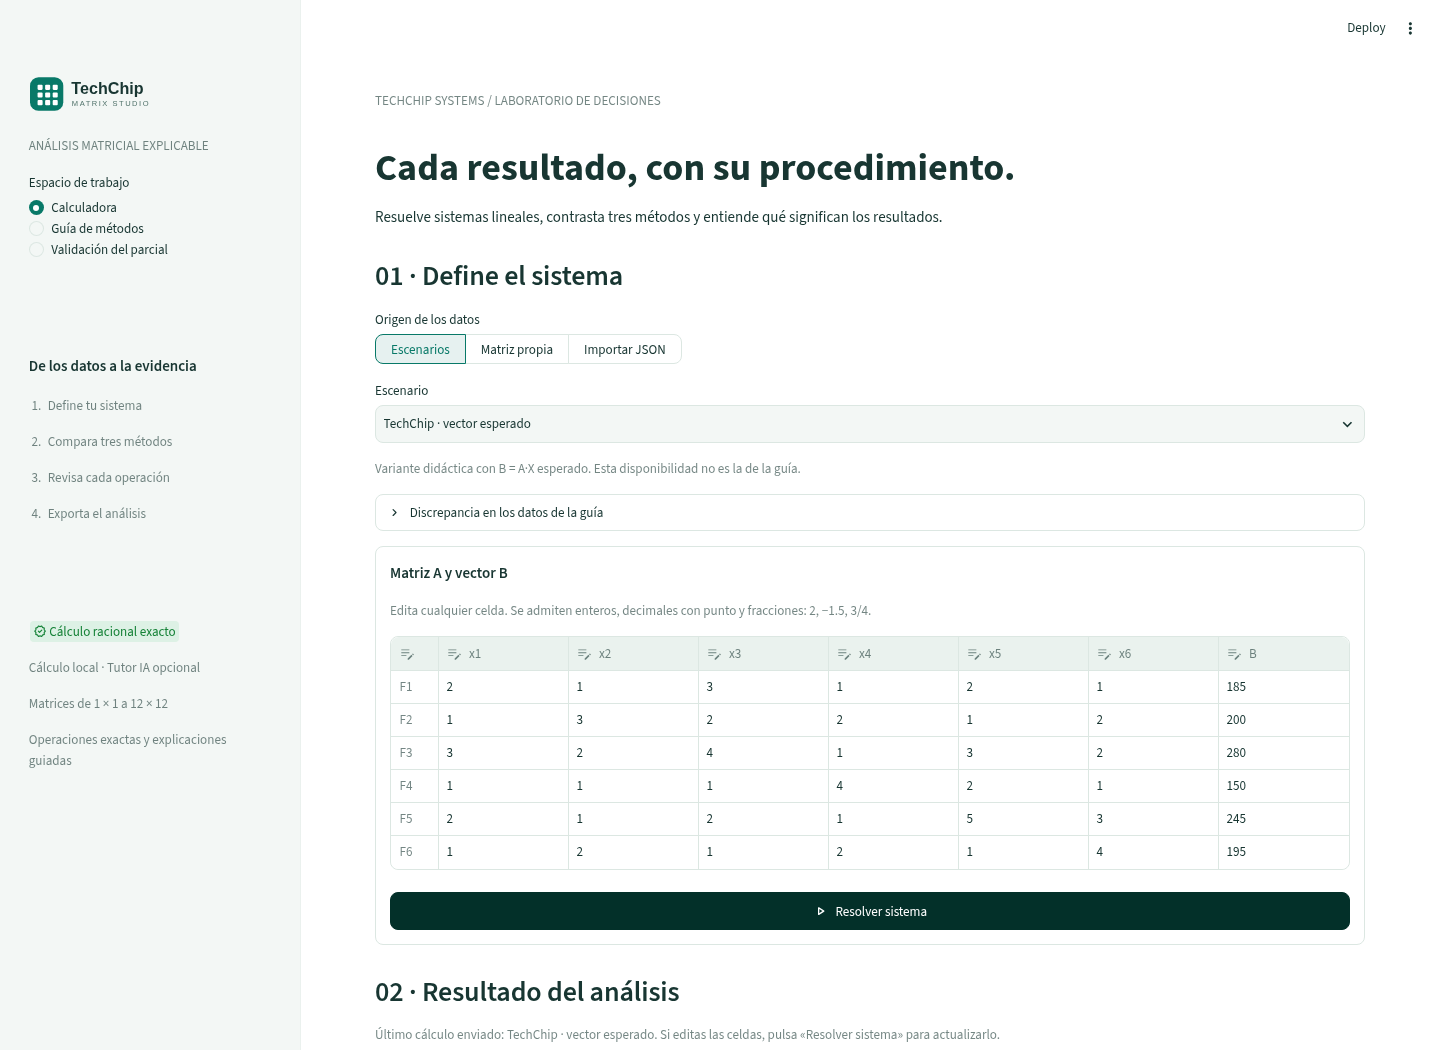
\includegraphics[width=\linewidth]{02_plan_compatible.png}\\[2pt]
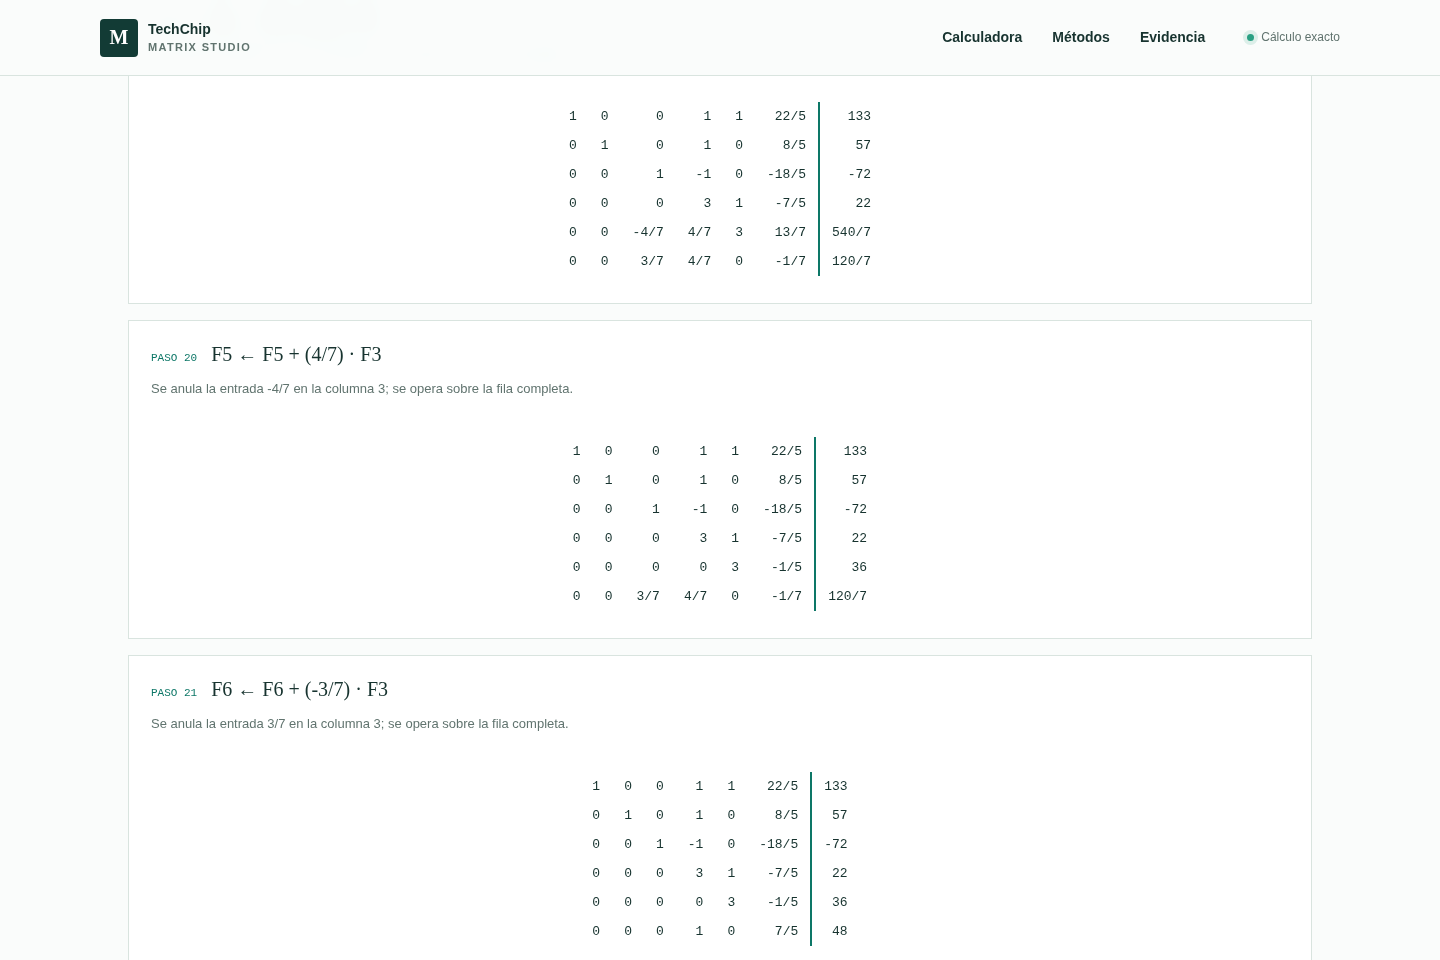
\includegraphics[width=\linewidth]{09_vercel_procedimiento.png}
\caption{Evidencia de ejecución: solución compatible y traza completa publicada en Vercel.}
\label{fig:evidencia}
\end{figure}

\section{Conclusiones}
La coincidencia exacta de tres algoritmos y el residuo nulo validan el caso compatible. La discrepancia de la guía es de datos, no del método: el vector esperado requiere otro $B$. El B original y la escasez producen soluciones algebraicas con componentes negativas y, por tanto, planes inviables bajo $X\ge0$. La singularidad distingue recursos redundantes de restricciones contradictorias. Para uso industrial se recomienda validar unidades, permitir holguras mediante desigualdades cuando corresponda e incorporar costos y demanda antes de hablar de optimización.

\begin{thebibliography}{9}
\bibitem{lay} D. C. Lay, S. R. Lay y J. J. McDonald, \emph{Linear Algebra and Its Applications}, 6.ª ed. Pearson, 2021.
\bibitem{strang} G. Strang, ``Gaussian elimination,'' MIT OpenCourseWare 18.06SC, 2011. [En línea]. Disponible: \url{https://ocw.mit.edu/courses/18-06sc-linear-algebra-fall-2011/}
\bibitem{python} Python Software Foundation, ``fractions --- Rational numbers.'' [En línea]. Disponible: \url{https://docs.python.org/3/library/fractions.html}
\bibitem{streamlit} Streamlit, ``Streamlit documentation.'' [En línea]. Disponible: \url{https://docs.streamlit.io/}
\bibitem{vercel} Vercel, ``Using the Python runtime with Vercel Functions.'' [En línea]. Disponible: \url{https://vercel.com/docs/functions/runtimes/python}
\bibitem{openai} OpenAI, ``Create a model response --- Responses API.'' [En línea]. Disponible: \url{https://developers.openai.com/api/reference/cli/resources/responses/methods/create}
\end{thebibliography}

\clearpage\onecolumn\appendices
\section{Eliminación de Gauss: procedimiento completo}
La secuencia contiene 25 estados registrados. Cada matriz es el estado posterior a la operación indicada.
\subsection*{Paso 1: Matriz aumentada inicial}
Punto de partida: [A | B]. La barra separa los coeficientes del bloque derecho, pero cada operación elemental se aplica a la fila completa para conservar un sistema equivalente.

\resizebox{0.97\textwidth}{!}{\(\left[\begin{array}{rrrrrr|r}2 & 1 & 3 & 1 & 2 & 1 & 185 \\ 1 & 3 & 2 & 2 & 1 & 2 & 200 \\ 3 & 2 & 4 & 1 & 3 & 2 & 280 \\ 1 & 1 & 1 & 4 & 2 & 1 & 150 \\ 2 & 1 & 2 & 1 & 5 & 3 & 245 \\ 1 & 2 & 1 & 2 & 1 & 4 & 195\end{array}\right]\)}

\medskip
\subsection*{Paso 2: F1 \(\leftrightarrow\) F3}
Pivoteo parcial en la columna 1: se coloca arriba el mayor valor absoluto disponible. Intercambiar ecuaciones solo cambia su orden, no el conjunto de soluciones; además evita dividir entre cero.

\resizebox{0.97\textwidth}{!}{\(\left[\begin{array}{rrrrrr|r}3 & 2 & 4 & 1 & 3 & 2 & 280 \\ 1 & 3 & 2 & 2 & 1 & 2 & 200 \\ 2 & 1 & 3 & 1 & 2 & 1 & 185 \\ 1 & 1 & 1 & 4 & 2 & 1 & 150 \\ 2 & 1 & 2 & 1 & 5 & 3 & 245 \\ 1 & 2 & 1 & 2 & 1 & 4 & 195\end{array}\right]\)}

\medskip
\subsection*{Paso 3: F2 \(\leftarrow\) F2 + (-1/3) \(\cdot\) F1}
El multiplicador es -(1)/(3) = -1/3; así, 1 + (-1/3)\(\cdot\)(3) = 0 en la columna 1. Sumar a una ecuación un múltiplo de otra es reversible y conserva exactamente las soluciones.

\resizebox{0.97\textwidth}{!}{\(\left[\begin{array}{rrrrrr|r}3 & 2 & 4 & 1 & 3 & 2 & 280 \\ 0 & \frac{7}{3} & \frac{2}{3} & \frac{5}{3} & 0 & \frac{4}{3} & \frac{320}{3} \\ 2 & 1 & 3 & 1 & 2 & 1 & 185 \\ 1 & 1 & 1 & 4 & 2 & 1 & 150 \\ 2 & 1 & 2 & 1 & 5 & 3 & 245 \\ 1 & 2 & 1 & 2 & 1 & 4 & 195\end{array}\right]\)}

\medskip
\subsection*{Paso 4: F3 \(\leftarrow\) F3 + (-2/3) \(\cdot\) F1}
El multiplicador es -(2)/(3) = -2/3; así, 2 + (-2/3)\(\cdot\)(3) = 0 en la columna 1. Sumar a una ecuación un múltiplo de otra es reversible y conserva exactamente las soluciones.

\resizebox{0.97\textwidth}{!}{\(\left[\begin{array}{rrrrrr|r}3 & 2 & 4 & 1 & 3 & 2 & 280 \\ 0 & \frac{7}{3} & \frac{2}{3} & \frac{5}{3} & 0 & \frac{4}{3} & \frac{320}{3} \\ 0 & -\frac{1}{3} & \frac{1}{3} & \frac{1}{3} & 0 & -\frac{1}{3} & -\frac{5}{3} \\ 1 & 1 & 1 & 4 & 2 & 1 & 150 \\ 2 & 1 & 2 & 1 & 5 & 3 & 245 \\ 1 & 2 & 1 & 2 & 1 & 4 & 195\end{array}\right]\)}

\medskip
\subsection*{Paso 5: F4 \(\leftarrow\) F4 + (-1/3) \(\cdot\) F1}
El multiplicador es -(1)/(3) = -1/3; así, 1 + (-1/3)\(\cdot\)(3) = 0 en la columna 1. Sumar a una ecuación un múltiplo de otra es reversible y conserva exactamente las soluciones.

\resizebox{0.97\textwidth}{!}{\(\left[\begin{array}{rrrrrr|r}3 & 2 & 4 & 1 & 3 & 2 & 280 \\ 0 & \frac{7}{3} & \frac{2}{3} & \frac{5}{3} & 0 & \frac{4}{3} & \frac{320}{3} \\ 0 & -\frac{1}{3} & \frac{1}{3} & \frac{1}{3} & 0 & -\frac{1}{3} & -\frac{5}{3} \\ 0 & \frac{1}{3} & -\frac{1}{3} & \frac{11}{3} & 1 & \frac{1}{3} & \frac{170}{3} \\ 2 & 1 & 2 & 1 & 5 & 3 & 245 \\ 1 & 2 & 1 & 2 & 1 & 4 & 195\end{array}\right]\)}

\medskip
\subsection*{Paso 6: F5 \(\leftarrow\) F5 + (-2/3) \(\cdot\) F1}
El multiplicador es -(2)/(3) = -2/3; así, 2 + (-2/3)\(\cdot\)(3) = 0 en la columna 1. Sumar a una ecuación un múltiplo de otra es reversible y conserva exactamente las soluciones.

\resizebox{0.97\textwidth}{!}{\(\left[\begin{array}{rrrrrr|r}3 & 2 & 4 & 1 & 3 & 2 & 280 \\ 0 & \frac{7}{3} & \frac{2}{3} & \frac{5}{3} & 0 & \frac{4}{3} & \frac{320}{3} \\ 0 & -\frac{1}{3} & \frac{1}{3} & \frac{1}{3} & 0 & -\frac{1}{3} & -\frac{5}{3} \\ 0 & \frac{1}{3} & -\frac{1}{3} & \frac{11}{3} & 1 & \frac{1}{3} & \frac{170}{3} \\ 0 & -\frac{1}{3} & -\frac{2}{3} & \frac{1}{3} & 3 & \frac{5}{3} & \frac{175}{3} \\ 1 & 2 & 1 & 2 & 1 & 4 & 195\end{array}\right]\)}

\medskip
\subsection*{Paso 7: F6 \(\leftarrow\) F6 + (-1/3) \(\cdot\) F1}
El multiplicador es -(1)/(3) = -1/3; así, 1 + (-1/3)\(\cdot\)(3) = 0 en la columna 1. Sumar a una ecuación un múltiplo de otra es reversible y conserva exactamente las soluciones.

\resizebox{0.97\textwidth}{!}{\(\left[\begin{array}{rrrrrr|r}3 & 2 & 4 & 1 & 3 & 2 & 280 \\ 0 & \frac{7}{3} & \frac{2}{3} & \frac{5}{3} & 0 & \frac{4}{3} & \frac{320}{3} \\ 0 & -\frac{1}{3} & \frac{1}{3} & \frac{1}{3} & 0 & -\frac{1}{3} & -\frac{5}{3} \\ 0 & \frac{1}{3} & -\frac{1}{3} & \frac{11}{3} & 1 & \frac{1}{3} & \frac{170}{3} \\ 0 & -\frac{1}{3} & -\frac{2}{3} & \frac{1}{3} & 3 & \frac{5}{3} & \frac{175}{3} \\ 0 & \frac{4}{3} & -\frac{1}{3} & \frac{5}{3} & 0 & \frac{10}{3} & \frac{305}{3}\end{array}\right]\)}

\medskip
\subsection*{Paso 8: F3 \(\leftarrow\) F3 + (1/7) \(\cdot\) F2}
El multiplicador es -(-1/3)/(7/3) = 1/7; así, -1/3 + (1/7)\(\cdot\)(7/3) = 0 en la columna 2. Sumar a una ecuación un múltiplo de otra es reversible y conserva exactamente las soluciones.

\resizebox{0.97\textwidth}{!}{\(\left[\begin{array}{rrrrrr|r}3 & 2 & 4 & 1 & 3 & 2 & 280 \\ 0 & \frac{7}{3} & \frac{2}{3} & \frac{5}{3} & 0 & \frac{4}{3} & \frac{320}{3} \\ 0 & 0 & \frac{3}{7} & \frac{4}{7} & 0 & -\frac{1}{7} & \frac{95}{7} \\ 0 & \frac{1}{3} & -\frac{1}{3} & \frac{11}{3} & 1 & \frac{1}{3} & \frac{170}{3} \\ 0 & -\frac{1}{3} & -\frac{2}{3} & \frac{1}{3} & 3 & \frac{5}{3} & \frac{175}{3} \\ 0 & \frac{4}{3} & -\frac{1}{3} & \frac{5}{3} & 0 & \frac{10}{3} & \frac{305}{3}\end{array}\right]\)}

\medskip
\subsection*{Paso 9: F4 \(\leftarrow\) F4 + (-1/7) \(\cdot\) F2}
El multiplicador es -(1/3)/(7/3) = -1/7; así, 1/3 + (-1/7)\(\cdot\)(7/3) = 0 en la columna 2. Sumar a una ecuación un múltiplo de otra es reversible y conserva exactamente las soluciones.

\resizebox{0.97\textwidth}{!}{\(\left[\begin{array}{rrrrrr|r}3 & 2 & 4 & 1 & 3 & 2 & 280 \\ 0 & \frac{7}{3} & \frac{2}{3} & \frac{5}{3} & 0 & \frac{4}{3} & \frac{320}{3} \\ 0 & 0 & \frac{3}{7} & \frac{4}{7} & 0 & -\frac{1}{7} & \frac{95}{7} \\ 0 & 0 & -\frac{3}{7} & \frac{24}{7} & 1 & \frac{1}{7} & \frac{290}{7} \\ 0 & -\frac{1}{3} & -\frac{2}{3} & \frac{1}{3} & 3 & \frac{5}{3} & \frac{175}{3} \\ 0 & \frac{4}{3} & -\frac{1}{3} & \frac{5}{3} & 0 & \frac{10}{3} & \frac{305}{3}\end{array}\right]\)}

\medskip
\subsection*{Paso 10: F5 \(\leftarrow\) F5 + (1/7) \(\cdot\) F2}
El multiplicador es -(-1/3)/(7/3) = 1/7; así, -1/3 + (1/7)\(\cdot\)(7/3) = 0 en la columna 2. Sumar a una ecuación un múltiplo de otra es reversible y conserva exactamente las soluciones.

\resizebox{0.97\textwidth}{!}{\(\left[\begin{array}{rrrrrr|r}3 & 2 & 4 & 1 & 3 & 2 & 280 \\ 0 & \frac{7}{3} & \frac{2}{3} & \frac{5}{3} & 0 & \frac{4}{3} & \frac{320}{3} \\ 0 & 0 & \frac{3}{7} & \frac{4}{7} & 0 & -\frac{1}{7} & \frac{95}{7} \\ 0 & 0 & -\frac{3}{7} & \frac{24}{7} & 1 & \frac{1}{7} & \frac{290}{7} \\ 0 & 0 & -\frac{4}{7} & \frac{4}{7} & 3 & \frac{13}{7} & \frac{515}{7} \\ 0 & \frac{4}{3} & -\frac{1}{3} & \frac{5}{3} & 0 & \frac{10}{3} & \frac{305}{3}\end{array}\right]\)}

\medskip
\subsection*{Paso 11: F6 \(\leftarrow\) F6 + (-4/7) \(\cdot\) F2}
El multiplicador es -(4/3)/(7/3) = -4/7; así, 4/3 + (-4/7)\(\cdot\)(7/3) = 0 en la columna 2. Sumar a una ecuación un múltiplo de otra es reversible y conserva exactamente las soluciones.

\resizebox{0.97\textwidth}{!}{\(\left[\begin{array}{rrrrrr|r}3 & 2 & 4 & 1 & 3 & 2 & 280 \\ 0 & \frac{7}{3} & \frac{2}{3} & \frac{5}{3} & 0 & \frac{4}{3} & \frac{320}{3} \\ 0 & 0 & \frac{3}{7} & \frac{4}{7} & 0 & -\frac{1}{7} & \frac{95}{7} \\ 0 & 0 & -\frac{3}{7} & \frac{24}{7} & 1 & \frac{1}{7} & \frac{290}{7} \\ 0 & 0 & -\frac{4}{7} & \frac{4}{7} & 3 & \frac{13}{7} & \frac{515}{7} \\ 0 & 0 & -\frac{5}{7} & \frac{5}{7} & 0 & \frac{18}{7} & \frac{285}{7}\end{array}\right]\)}

\medskip
\subsection*{Paso 12: F3 \(\leftrightarrow\) F6}
Pivoteo parcial en la columna 3: se coloca arriba el mayor valor absoluto disponible. Intercambiar ecuaciones solo cambia su orden, no el conjunto de soluciones; además evita dividir entre cero.

\resizebox{0.97\textwidth}{!}{\(\left[\begin{array}{rrrrrr|r}3 & 2 & 4 & 1 & 3 & 2 & 280 \\ 0 & \frac{7}{3} & \frac{2}{3} & \frac{5}{3} & 0 & \frac{4}{3} & \frac{320}{3} \\ 0 & 0 & -\frac{5}{7} & \frac{5}{7} & 0 & \frac{18}{7} & \frac{285}{7} \\ 0 & 0 & -\frac{3}{7} & \frac{24}{7} & 1 & \frac{1}{7} & \frac{290}{7} \\ 0 & 0 & -\frac{4}{7} & \frac{4}{7} & 3 & \frac{13}{7} & \frac{515}{7} \\ 0 & 0 & \frac{3}{7} & \frac{4}{7} & 0 & -\frac{1}{7} & \frac{95}{7}\end{array}\right]\)}

\medskip
\subsection*{Paso 13: F4 \(\leftarrow\) F4 + (-3/5) \(\cdot\) F3}
El multiplicador es -(-3/7)/(-5/7) = -3/5; así, -3/7 + (-3/5)\(\cdot\)(-5/7) = 0 en la columna 3. Sumar a una ecuación un múltiplo de otra es reversible y conserva exactamente las soluciones.

\resizebox{0.97\textwidth}{!}{\(\left[\begin{array}{rrrrrr|r}3 & 2 & 4 & 1 & 3 & 2 & 280 \\ 0 & \frac{7}{3} & \frac{2}{3} & \frac{5}{3} & 0 & \frac{4}{3} & \frac{320}{3} \\ 0 & 0 & -\frac{5}{7} & \frac{5}{7} & 0 & \frac{18}{7} & \frac{285}{7} \\ 0 & 0 & 0 & 3 & 1 & -\frac{7}{5} & 17 \\ 0 & 0 & -\frac{4}{7} & \frac{4}{7} & 3 & \frac{13}{7} & \frac{515}{7} \\ 0 & 0 & \frac{3}{7} & \frac{4}{7} & 0 & -\frac{1}{7} & \frac{95}{7}\end{array}\right]\)}

\medskip
\subsection*{Paso 14: F5 \(\leftarrow\) F5 + (-4/5) \(\cdot\) F3}
El multiplicador es -(-4/7)/(-5/7) = -4/5; así, -4/7 + (-4/5)\(\cdot\)(-5/7) = 0 en la columna 3. Sumar a una ecuación un múltiplo de otra es reversible y conserva exactamente las soluciones.

\resizebox{0.97\textwidth}{!}{\(\left[\begin{array}{rrrrrr|r}3 & 2 & 4 & 1 & 3 & 2 & 280 \\ 0 & \frac{7}{3} & \frac{2}{3} & \frac{5}{3} & 0 & \frac{4}{3} & \frac{320}{3} \\ 0 & 0 & -\frac{5}{7} & \frac{5}{7} & 0 & \frac{18}{7} & \frac{285}{7} \\ 0 & 0 & 0 & 3 & 1 & -\frac{7}{5} & 17 \\ 0 & 0 & 0 & 0 & 3 & -\frac{1}{5} & 41 \\ 0 & 0 & \frac{3}{7} & \frac{4}{7} & 0 & -\frac{1}{7} & \frac{95}{7}\end{array}\right]\)}

\medskip
\subsection*{Paso 15: F6 \(\leftarrow\) F6 + (3/5) \(\cdot\) F3}
El multiplicador es -(3/7)/(-5/7) = 3/5; así, 3/7 + (3/5)\(\cdot\)(-5/7) = 0 en la columna 3. Sumar a una ecuación un múltiplo de otra es reversible y conserva exactamente las soluciones.

\resizebox{0.97\textwidth}{!}{\(\left[\begin{array}{rrrrrr|r}3 & 2 & 4 & 1 & 3 & 2 & 280 \\ 0 & \frac{7}{3} & \frac{2}{3} & \frac{5}{3} & 0 & \frac{4}{3} & \frac{320}{3} \\ 0 & 0 & -\frac{5}{7} & \frac{5}{7} & 0 & \frac{18}{7} & \frac{285}{7} \\ 0 & 0 & 0 & 3 & 1 & -\frac{7}{5} & 17 \\ 0 & 0 & 0 & 0 & 3 & -\frac{1}{5} & 41 \\ 0 & 0 & 0 & 1 & 0 & \frac{7}{5} & 38\end{array}\right]\)}

\medskip
\subsection*{Paso 16: F6 \(\leftarrow\) F6 + (-1/3) \(\cdot\) F4}
El multiplicador es -(1)/(3) = -1/3; así, 1 + (-1/3)\(\cdot\)(3) = 0 en la columna 4. Sumar a una ecuación un múltiplo de otra es reversible y conserva exactamente las soluciones.

\resizebox{0.97\textwidth}{!}{\(\left[\begin{array}{rrrrrr|r}3 & 2 & 4 & 1 & 3 & 2 & 280 \\ 0 & \frac{7}{3} & \frac{2}{3} & \frac{5}{3} & 0 & \frac{4}{3} & \frac{320}{3} \\ 0 & 0 & -\frac{5}{7} & \frac{5}{7} & 0 & \frac{18}{7} & \frac{285}{7} \\ 0 & 0 & 0 & 3 & 1 & -\frac{7}{5} & 17 \\ 0 & 0 & 0 & 0 & 3 & -\frac{1}{5} & 41 \\ 0 & 0 & 0 & 0 & -\frac{1}{3} & \frac{28}{15} & \frac{97}{3}\end{array}\right]\)}

\medskip
\subsection*{Paso 17: F6 \(\leftarrow\) F6 + (1/9) \(\cdot\) F5}
El multiplicador es -(-1/3)/(3) = 1/9; así, -1/3 + (1/9)\(\cdot\)(3) = 0 en la columna 5. Sumar a una ecuación un múltiplo de otra es reversible y conserva exactamente las soluciones.

\resizebox{0.97\textwidth}{!}{\(\left[\begin{array}{rrrrrr|r}3 & 2 & 4 & 1 & 3 & 2 & 280 \\ 0 & \frac{7}{3} & \frac{2}{3} & \frac{5}{3} & 0 & \frac{4}{3} & \frac{320}{3} \\ 0 & 0 & -\frac{5}{7} & \frac{5}{7} & 0 & \frac{18}{7} & \frac{285}{7} \\ 0 & 0 & 0 & 3 & 1 & -\frac{7}{5} & 17 \\ 0 & 0 & 0 & 0 & 3 & -\frac{1}{5} & 41 \\ 0 & 0 & 0 & 0 & 0 & \frac{83}{45} & \frac{332}{9}\end{array}\right]\)}

\medskip
\subsection*{Paso 18: det(A) = -83}
2 intercambio(s). Las sumas de filas conservan el determinante. det(A) = (-1)\textasciicircum{}2 \(\cdot\) (3) \(\cdot\) (7/3) \(\cdot\) (-5/7) \(\cdot\) (3) \(\cdot\) (3) \(\cdot\) (83/45) = -83.

\resizebox{0.97\textwidth}{!}{\(\left[\begin{array}{rrrrrr|r}3 & 2 & 4 & 1 & 3 & 2 & 280 \\ 0 & \frac{7}{3} & \frac{2}{3} & \frac{5}{3} & 0 & \frac{4}{3} & \frac{320}{3} \\ 0 & 0 & -\frac{5}{7} & \frac{5}{7} & 0 & \frac{18}{7} & \frac{285}{7} \\ 0 & 0 & 0 & 3 & 1 & -\frac{7}{5} & 17 \\ 0 & 0 & 0 & 0 & 3 & -\frac{1}{5} & 41 \\ 0 & 0 & 0 & 0 & 0 & \frac{83}{45} & \frac{332}{9}\end{array}\right]\)}

\medskip
\subsection*{Paso 19: Matriz triangular superior U}
La eliminación terminó: debajo de cada pivote hay ceros. Ahora se resuelve U\(\cdot\)X = C desde la última ecuación hacia la primera, porque cada fila solo depende de variables ya conocidas.

\resizebox{0.97\textwidth}{!}{\(\left[\begin{array}{rrrrrr|r}3 & 2 & 4 & 1 & 3 & 2 & 280 \\ 0 & \frac{7}{3} & \frac{2}{3} & \frac{5}{3} & 0 & \frac{4}{3} & \frac{320}{3} \\ 0 & 0 & -\frac{5}{7} & \frac{5}{7} & 0 & \frac{18}{7} & \frac{285}{7} \\ 0 & 0 & 0 & 3 & 1 & -\frac{7}{5} & 17 \\ 0 & 0 & 0 & 0 & 3 & -\frac{1}{5} & 41 \\ 0 & 0 & 0 & 0 & 0 & \frac{83}{45} & \frac{332}{9}\end{array}\right]\)}

\medskip
\subsection*{Paso 20: x6 = (332/9 - (0)) / (83/45) = 20}
En la fila 6 se pasan al lado derecho los términos ya conocidos y se divide entre el coeficiente de x6. El valor se conserva como fracción exacta.

\resizebox{0.97\textwidth}{!}{\(\left[\begin{array}{rrrrrr|r}3 & 2 & 4 & 1 & 3 & 2 & 280 \\ 0 & \frac{7}{3} & \frac{2}{3} & \frac{5}{3} & 0 & \frac{4}{3} & \frac{320}{3} \\ 0 & 0 & -\frac{5}{7} & \frac{5}{7} & 0 & \frac{18}{7} & \frac{285}{7} \\ 0 & 0 & 0 & 3 & 1 & -\frac{7}{5} & 17 \\ 0 & 0 & 0 & 0 & 3 & -\frac{1}{5} & 41 \\ 0 & 0 & 0 & 0 & 0 & \frac{83}{45} & \frac{332}{9}\end{array}\right]\)}

\medskip
\subsection*{Paso 21: x5 = (41 - ((-1/5)\(\cdot\)(20))) / (3) = 15}
En la fila 5 se pasan al lado derecho los términos ya conocidos y se divide entre el coeficiente de x5. El valor se conserva como fracción exacta.

\resizebox{0.97\textwidth}{!}{\(\left[\begin{array}{rrrrrr|r}3 & 2 & 4 & 1 & 3 & 2 & 280 \\ 0 & \frac{7}{3} & \frac{2}{3} & \frac{5}{3} & 0 & \frac{4}{3} & \frac{320}{3} \\ 0 & 0 & -\frac{5}{7} & \frac{5}{7} & 0 & \frac{18}{7} & \frac{285}{7} \\ 0 & 0 & 0 & 3 & 1 & -\frac{7}{5} & 17 \\ 0 & 0 & 0 & 0 & 3 & -\frac{1}{5} & 41 \\ 0 & 0 & 0 & 0 & 0 & \frac{83}{45} & \frac{332}{9}\end{array}\right]\)}

\medskip
\subsection*{Paso 22: x4 = (17 - ((1)\(\cdot\)(15) + (-7/5)\(\cdot\)(20))) / (3) = 10}
En la fila 4 se pasan al lado derecho los términos ya conocidos y se divide entre el coeficiente de x4. El valor se conserva como fracción exacta.

\resizebox{0.97\textwidth}{!}{\(\left[\begin{array}{rrrrrr|r}3 & 2 & 4 & 1 & 3 & 2 & 280 \\ 0 & \frac{7}{3} & \frac{2}{3} & \frac{5}{3} & 0 & \frac{4}{3} & \frac{320}{3} \\ 0 & 0 & -\frac{5}{7} & \frac{5}{7} & 0 & \frac{18}{7} & \frac{285}{7} \\ 0 & 0 & 0 & 3 & 1 & -\frac{7}{5} & 17 \\ 0 & 0 & 0 & 0 & 3 & -\frac{1}{5} & 41 \\ 0 & 0 & 0 & 0 & 0 & \frac{83}{45} & \frac{332}{9}\end{array}\right]\)}

\medskip
\subsection*{Paso 23: x3 = (285/7 - ((5/7)\(\cdot\)(10) + (0)\(\cdot\)(15) + (18/7)\(\cdot\)(20))) / (-5/7) = 25}
En la fila 3 se pasan al lado derecho los términos ya conocidos y se divide entre el coeficiente de x3. El valor se conserva como fracción exacta.

\resizebox{0.97\textwidth}{!}{\(\left[\begin{array}{rrrrrr|r}3 & 2 & 4 & 1 & 3 & 2 & 280 \\ 0 & \frac{7}{3} & \frac{2}{3} & \frac{5}{3} & 0 & \frac{4}{3} & \frac{320}{3} \\ 0 & 0 & -\frac{5}{7} & \frac{5}{7} & 0 & \frac{18}{7} & \frac{285}{7} \\ 0 & 0 & 0 & 3 & 1 & -\frac{7}{5} & 17 \\ 0 & 0 & 0 & 0 & 3 & -\frac{1}{5} & 41 \\ 0 & 0 & 0 & 0 & 0 & \frac{83}{45} & \frac{332}{9}\end{array}\right]\)}

\medskip
\subsection*{Paso 24: x2 = (320/3 - ((2/3)\(\cdot\)(25) + (5/3)\(\cdot\)(10) + (0)\(\cdot\)(15) + (4/3)\(\cdot\)(20))) / (7/3) = 20}
En la fila 2 se pasan al lado derecho los términos ya conocidos y se divide entre el coeficiente de x2. El valor se conserva como fracción exacta.

\resizebox{0.97\textwidth}{!}{\(\left[\begin{array}{rrrrrr|r}3 & 2 & 4 & 1 & 3 & 2 & 280 \\ 0 & \frac{7}{3} & \frac{2}{3} & \frac{5}{3} & 0 & \frac{4}{3} & \frac{320}{3} \\ 0 & 0 & -\frac{5}{7} & \frac{5}{7} & 0 & \frac{18}{7} & \frac{285}{7} \\ 0 & 0 & 0 & 3 & 1 & -\frac{7}{5} & 17 \\ 0 & 0 & 0 & 0 & 3 & -\frac{1}{5} & 41 \\ 0 & 0 & 0 & 0 & 0 & \frac{83}{45} & \frac{332}{9}\end{array}\right]\)}

\medskip
\subsection*{Paso 25: x1 = (280 - ((2)\(\cdot\)(20) + (4)\(\cdot\)(25) + (1)\(\cdot\)(10) + (3)\(\cdot\)(15) + (2)\(\cdot\)(20))) / (3) = 15}
En la fila 1 se pasan al lado derecho los términos ya conocidos y se divide entre el coeficiente de x1. El valor se conserva como fracción exacta.

\resizebox{0.97\textwidth}{!}{\(\left[\begin{array}{rrrrrr|r}3 & 2 & 4 & 1 & 3 & 2 & 280 \\ 0 & \frac{7}{3} & \frac{2}{3} & \frac{5}{3} & 0 & \frac{4}{3} & \frac{320}{3} \\ 0 & 0 & -\frac{5}{7} & \frac{5}{7} & 0 & \frac{18}{7} & \frac{285}{7} \\ 0 & 0 & 0 & 3 & 1 & -\frac{7}{5} & 17 \\ 0 & 0 & 0 & 0 & 3 & -\frac{1}{5} & 41 \\ 0 & 0 & 0 & 0 & 0 & \frac{83}{45} & \frac{332}{9}\end{array}\right]\)}

\medskip
\section{Gauss--Jordan: procedimiento completo}
La secuencia contiene 39 estados registrados. Cada matriz es el estado posterior a la operación indicada.
\subsection*{Paso 1: Matriz aumentada inicial}
Punto de partida: [A | B]. La barra separa los coeficientes del bloque derecho, pero cada operación elemental se aplica a la fila completa para conservar un sistema equivalente.

\resizebox{0.97\textwidth}{!}{\(\left[\begin{array}{rrrrrr|r}2 & 1 & 3 & 1 & 2 & 1 & 185 \\ 1 & 3 & 2 & 2 & 1 & 2 & 200 \\ 3 & 2 & 4 & 1 & 3 & 2 & 280 \\ 1 & 1 & 1 & 4 & 2 & 1 & 150 \\ 2 & 1 & 2 & 1 & 5 & 3 & 245 \\ 1 & 2 & 1 & 2 & 1 & 4 & 195\end{array}\right]\)}

\medskip
\subsection*{Paso 2: F1 \(\leftrightarrow\) F3}
Pivoteo parcial en la columna 1: se coloca arriba el mayor valor absoluto disponible. Intercambiar ecuaciones solo cambia su orden, no el conjunto de soluciones; además evita dividir entre cero.

\resizebox{0.97\textwidth}{!}{\(\left[\begin{array}{rrrrrr|r}3 & 2 & 4 & 1 & 3 & 2 & 280 \\ 1 & 3 & 2 & 2 & 1 & 2 & 200 \\ 2 & 1 & 3 & 1 & 2 & 1 & 185 \\ 1 & 1 & 1 & 4 & 2 & 1 & 150 \\ 2 & 1 & 2 & 1 & 5 & 3 & 245 \\ 1 & 2 & 1 & 2 & 1 & 4 & 195\end{array}\right]\)}

\medskip
\subsection*{Paso 3: F1 \(\leftarrow\) (1/3) \(\cdot\) F1}
Se divide toda la fila entre el pivote 3, por eso el pivote se convierte en 1. Multiplicar una ecuación por un número distinto de cero produce una ecuación equivalente.

\resizebox{0.97\textwidth}{!}{\(\left[\begin{array}{rrrrrr|r}1 & \frac{2}{3} & \frac{4}{3} & \frac{1}{3} & 1 & \frac{2}{3} & \frac{280}{3} \\ 1 & 3 & 2 & 2 & 1 & 2 & 200 \\ 2 & 1 & 3 & 1 & 2 & 1 & 185 \\ 1 & 1 & 1 & 4 & 2 & 1 & 150 \\ 2 & 1 & 2 & 1 & 5 & 3 & 245 \\ 1 & 2 & 1 & 2 & 1 & 4 & 195\end{array}\right]\)}

\medskip
\subsection*{Paso 4: F2 \(\leftarrow\) F2 + (-1) \(\cdot\) F1}
El multiplicador es -(1)/(1) = -1; así, 1 + (-1)\(\cdot\)(1) = 0 en la columna 1. Sumar a una ecuación un múltiplo de otra es reversible y conserva exactamente las soluciones.

\resizebox{0.97\textwidth}{!}{\(\left[\begin{array}{rrrrrr|r}1 & \frac{2}{3} & \frac{4}{3} & \frac{1}{3} & 1 & \frac{2}{3} & \frac{280}{3} \\ 0 & \frac{7}{3} & \frac{2}{3} & \frac{5}{3} & 0 & \frac{4}{3} & \frac{320}{3} \\ 2 & 1 & 3 & 1 & 2 & 1 & 185 \\ 1 & 1 & 1 & 4 & 2 & 1 & 150 \\ 2 & 1 & 2 & 1 & 5 & 3 & 245 \\ 1 & 2 & 1 & 2 & 1 & 4 & 195\end{array}\right]\)}

\medskip
\subsection*{Paso 5: F3 \(\leftarrow\) F3 + (-2) \(\cdot\) F1}
El multiplicador es -(2)/(1) = -2; así, 2 + (-2)\(\cdot\)(1) = 0 en la columna 1. Sumar a una ecuación un múltiplo de otra es reversible y conserva exactamente las soluciones.

\resizebox{0.97\textwidth}{!}{\(\left[\begin{array}{rrrrrr|r}1 & \frac{2}{3} & \frac{4}{3} & \frac{1}{3} & 1 & \frac{2}{3} & \frac{280}{3} \\ 0 & \frac{7}{3} & \frac{2}{3} & \frac{5}{3} & 0 & \frac{4}{3} & \frac{320}{3} \\ 0 & -\frac{1}{3} & \frac{1}{3} & \frac{1}{3} & 0 & -\frac{1}{3} & -\frac{5}{3} \\ 1 & 1 & 1 & 4 & 2 & 1 & 150 \\ 2 & 1 & 2 & 1 & 5 & 3 & 245 \\ 1 & 2 & 1 & 2 & 1 & 4 & 195\end{array}\right]\)}

\medskip
\subsection*{Paso 6: F4 \(\leftarrow\) F4 + (-1) \(\cdot\) F1}
El multiplicador es -(1)/(1) = -1; así, 1 + (-1)\(\cdot\)(1) = 0 en la columna 1. Sumar a una ecuación un múltiplo de otra es reversible y conserva exactamente las soluciones.

\resizebox{0.97\textwidth}{!}{\(\left[\begin{array}{rrrrrr|r}1 & \frac{2}{3} & \frac{4}{3} & \frac{1}{3} & 1 & \frac{2}{3} & \frac{280}{3} \\ 0 & \frac{7}{3} & \frac{2}{3} & \frac{5}{3} & 0 & \frac{4}{3} & \frac{320}{3} \\ 0 & -\frac{1}{3} & \frac{1}{3} & \frac{1}{3} & 0 & -\frac{1}{3} & -\frac{5}{3} \\ 0 & \frac{1}{3} & -\frac{1}{3} & \frac{11}{3} & 1 & \frac{1}{3} & \frac{170}{3} \\ 2 & 1 & 2 & 1 & 5 & 3 & 245 \\ 1 & 2 & 1 & 2 & 1 & 4 & 195\end{array}\right]\)}

\medskip
\subsection*{Paso 7: F5 \(\leftarrow\) F5 + (-2) \(\cdot\) F1}
El multiplicador es -(2)/(1) = -2; así, 2 + (-2)\(\cdot\)(1) = 0 en la columna 1. Sumar a una ecuación un múltiplo de otra es reversible y conserva exactamente las soluciones.

\resizebox{0.97\textwidth}{!}{\(\left[\begin{array}{rrrrrr|r}1 & \frac{2}{3} & \frac{4}{3} & \frac{1}{3} & 1 & \frac{2}{3} & \frac{280}{3} \\ 0 & \frac{7}{3} & \frac{2}{3} & \frac{5}{3} & 0 & \frac{4}{3} & \frac{320}{3} \\ 0 & -\frac{1}{3} & \frac{1}{3} & \frac{1}{3} & 0 & -\frac{1}{3} & -\frac{5}{3} \\ 0 & \frac{1}{3} & -\frac{1}{3} & \frac{11}{3} & 1 & \frac{1}{3} & \frac{170}{3} \\ 0 & -\frac{1}{3} & -\frac{2}{3} & \frac{1}{3} & 3 & \frac{5}{3} & \frac{175}{3} \\ 1 & 2 & 1 & 2 & 1 & 4 & 195\end{array}\right]\)}

\medskip
\subsection*{Paso 8: F6 \(\leftarrow\) F6 + (-1) \(\cdot\) F1}
El multiplicador es -(1)/(1) = -1; así, 1 + (-1)\(\cdot\)(1) = 0 en la columna 1. Sumar a una ecuación un múltiplo de otra es reversible y conserva exactamente las soluciones.

\resizebox{0.97\textwidth}{!}{\(\left[\begin{array}{rrrrrr|r}1 & \frac{2}{3} & \frac{4}{3} & \frac{1}{3} & 1 & \frac{2}{3} & \frac{280}{3} \\ 0 & \frac{7}{3} & \frac{2}{3} & \frac{5}{3} & 0 & \frac{4}{3} & \frac{320}{3} \\ 0 & -\frac{1}{3} & \frac{1}{3} & \frac{1}{3} & 0 & -\frac{1}{3} & -\frac{5}{3} \\ 0 & \frac{1}{3} & -\frac{1}{3} & \frac{11}{3} & 1 & \frac{1}{3} & \frac{170}{3} \\ 0 & -\frac{1}{3} & -\frac{2}{3} & \frac{1}{3} & 3 & \frac{5}{3} & \frac{175}{3} \\ 0 & \frac{4}{3} & -\frac{1}{3} & \frac{5}{3} & 0 & \frac{10}{3} & \frac{305}{3}\end{array}\right]\)}

\medskip
\subsection*{Paso 9: F2 \(\leftarrow\) (3/7) \(\cdot\) F2}
Se divide toda la fila entre el pivote 7/3, por eso el pivote se convierte en 1. Multiplicar una ecuación por un número distinto de cero produce una ecuación equivalente.

\resizebox{0.97\textwidth}{!}{\(\left[\begin{array}{rrrrrr|r}1 & \frac{2}{3} & \frac{4}{3} & \frac{1}{3} & 1 & \frac{2}{3} & \frac{280}{3} \\ 0 & 1 & \frac{2}{7} & \frac{5}{7} & 0 & \frac{4}{7} & \frac{320}{7} \\ 0 & -\frac{1}{3} & \frac{1}{3} & \frac{1}{3} & 0 & -\frac{1}{3} & -\frac{5}{3} \\ 0 & \frac{1}{3} & -\frac{1}{3} & \frac{11}{3} & 1 & \frac{1}{3} & \frac{170}{3} \\ 0 & -\frac{1}{3} & -\frac{2}{3} & \frac{1}{3} & 3 & \frac{5}{3} & \frac{175}{3} \\ 0 & \frac{4}{3} & -\frac{1}{3} & \frac{5}{3} & 0 & \frac{10}{3} & \frac{305}{3}\end{array}\right]\)}

\medskip
\subsection*{Paso 10: F1 \(\leftarrow\) F1 + (-2/3) \(\cdot\) F2}
El multiplicador es -(2/3)/(1) = -2/3; así, 2/3 + (-2/3)\(\cdot\)(1) = 0 en la columna 2. Sumar a una ecuación un múltiplo de otra es reversible y conserva exactamente las soluciones.

\resizebox{0.97\textwidth}{!}{\(\left[\begin{array}{rrrrrr|r}1 & 0 & \frac{8}{7} & -\frac{1}{7} & 1 & \frac{2}{7} & \frac{440}{7} \\ 0 & 1 & \frac{2}{7} & \frac{5}{7} & 0 & \frac{4}{7} & \frac{320}{7} \\ 0 & -\frac{1}{3} & \frac{1}{3} & \frac{1}{3} & 0 & -\frac{1}{3} & -\frac{5}{3} \\ 0 & \frac{1}{3} & -\frac{1}{3} & \frac{11}{3} & 1 & \frac{1}{3} & \frac{170}{3} \\ 0 & -\frac{1}{3} & -\frac{2}{3} & \frac{1}{3} & 3 & \frac{5}{3} & \frac{175}{3} \\ 0 & \frac{4}{3} & -\frac{1}{3} & \frac{5}{3} & 0 & \frac{10}{3} & \frac{305}{3}\end{array}\right]\)}

\medskip
\subsection*{Paso 11: F3 \(\leftarrow\) F3 + (1/3) \(\cdot\) F2}
El multiplicador es -(-1/3)/(1) = 1/3; así, -1/3 + (1/3)\(\cdot\)(1) = 0 en la columna 2. Sumar a una ecuación un múltiplo de otra es reversible y conserva exactamente las soluciones.

\resizebox{0.97\textwidth}{!}{\(\left[\begin{array}{rrrrrr|r}1 & 0 & \frac{8}{7} & -\frac{1}{7} & 1 & \frac{2}{7} & \frac{440}{7} \\ 0 & 1 & \frac{2}{7} & \frac{5}{7} & 0 & \frac{4}{7} & \frac{320}{7} \\ 0 & 0 & \frac{3}{7} & \frac{4}{7} & 0 & -\frac{1}{7} & \frac{95}{7} \\ 0 & \frac{1}{3} & -\frac{1}{3} & \frac{11}{3} & 1 & \frac{1}{3} & \frac{170}{3} \\ 0 & -\frac{1}{3} & -\frac{2}{3} & \frac{1}{3} & 3 & \frac{5}{3} & \frac{175}{3} \\ 0 & \frac{4}{3} & -\frac{1}{3} & \frac{5}{3} & 0 & \frac{10}{3} & \frac{305}{3}\end{array}\right]\)}

\medskip
\subsection*{Paso 12: F4 \(\leftarrow\) F4 + (-1/3) \(\cdot\) F2}
El multiplicador es -(1/3)/(1) = -1/3; así, 1/3 + (-1/3)\(\cdot\)(1) = 0 en la columna 2. Sumar a una ecuación un múltiplo de otra es reversible y conserva exactamente las soluciones.

\resizebox{0.97\textwidth}{!}{\(\left[\begin{array}{rrrrrr|r}1 & 0 & \frac{8}{7} & -\frac{1}{7} & 1 & \frac{2}{7} & \frac{440}{7} \\ 0 & 1 & \frac{2}{7} & \frac{5}{7} & 0 & \frac{4}{7} & \frac{320}{7} \\ 0 & 0 & \frac{3}{7} & \frac{4}{7} & 0 & -\frac{1}{7} & \frac{95}{7} \\ 0 & 0 & -\frac{3}{7} & \frac{24}{7} & 1 & \frac{1}{7} & \frac{290}{7} \\ 0 & -\frac{1}{3} & -\frac{2}{3} & \frac{1}{3} & 3 & \frac{5}{3} & \frac{175}{3} \\ 0 & \frac{4}{3} & -\frac{1}{3} & \frac{5}{3} & 0 & \frac{10}{3} & \frac{305}{3}\end{array}\right]\)}

\medskip
\subsection*{Paso 13: F5 \(\leftarrow\) F5 + (1/3) \(\cdot\) F2}
El multiplicador es -(-1/3)/(1) = 1/3; así, -1/3 + (1/3)\(\cdot\)(1) = 0 en la columna 2. Sumar a una ecuación un múltiplo de otra es reversible y conserva exactamente las soluciones.

\resizebox{0.97\textwidth}{!}{\(\left[\begin{array}{rrrrrr|r}1 & 0 & \frac{8}{7} & -\frac{1}{7} & 1 & \frac{2}{7} & \frac{440}{7} \\ 0 & 1 & \frac{2}{7} & \frac{5}{7} & 0 & \frac{4}{7} & \frac{320}{7} \\ 0 & 0 & \frac{3}{7} & \frac{4}{7} & 0 & -\frac{1}{7} & \frac{95}{7} \\ 0 & 0 & -\frac{3}{7} & \frac{24}{7} & 1 & \frac{1}{7} & \frac{290}{7} \\ 0 & 0 & -\frac{4}{7} & \frac{4}{7} & 3 & \frac{13}{7} & \frac{515}{7} \\ 0 & \frac{4}{3} & -\frac{1}{3} & \frac{5}{3} & 0 & \frac{10}{3} & \frac{305}{3}\end{array}\right]\)}

\medskip
\subsection*{Paso 14: F6 \(\leftarrow\) F6 + (-4/3) \(\cdot\) F2}
El multiplicador es -(4/3)/(1) = -4/3; así, 4/3 + (-4/3)\(\cdot\)(1) = 0 en la columna 2. Sumar a una ecuación un múltiplo de otra es reversible y conserva exactamente las soluciones.

\resizebox{0.97\textwidth}{!}{\(\left[\begin{array}{rrrrrr|r}1 & 0 & \frac{8}{7} & -\frac{1}{7} & 1 & \frac{2}{7} & \frac{440}{7} \\ 0 & 1 & \frac{2}{7} & \frac{5}{7} & 0 & \frac{4}{7} & \frac{320}{7} \\ 0 & 0 & \frac{3}{7} & \frac{4}{7} & 0 & -\frac{1}{7} & \frac{95}{7} \\ 0 & 0 & -\frac{3}{7} & \frac{24}{7} & 1 & \frac{1}{7} & \frac{290}{7} \\ 0 & 0 & -\frac{4}{7} & \frac{4}{7} & 3 & \frac{13}{7} & \frac{515}{7} \\ 0 & 0 & -\frac{5}{7} & \frac{5}{7} & 0 & \frac{18}{7} & \frac{285}{7}\end{array}\right]\)}

\medskip
\subsection*{Paso 15: F3 \(\leftrightarrow\) F6}
Pivoteo parcial en la columna 3: se coloca arriba el mayor valor absoluto disponible. Intercambiar ecuaciones solo cambia su orden, no el conjunto de soluciones; además evita dividir entre cero.

\resizebox{0.97\textwidth}{!}{\(\left[\begin{array}{rrrrrr|r}1 & 0 & \frac{8}{7} & -\frac{1}{7} & 1 & \frac{2}{7} & \frac{440}{7} \\ 0 & 1 & \frac{2}{7} & \frac{5}{7} & 0 & \frac{4}{7} & \frac{320}{7} \\ 0 & 0 & -\frac{5}{7} & \frac{5}{7} & 0 & \frac{18}{7} & \frac{285}{7} \\ 0 & 0 & -\frac{3}{7} & \frac{24}{7} & 1 & \frac{1}{7} & \frac{290}{7} \\ 0 & 0 & -\frac{4}{7} & \frac{4}{7} & 3 & \frac{13}{7} & \frac{515}{7} \\ 0 & 0 & \frac{3}{7} & \frac{4}{7} & 0 & -\frac{1}{7} & \frac{95}{7}\end{array}\right]\)}

\medskip
\subsection*{Paso 16: F3 \(\leftarrow\) (-7/5) \(\cdot\) F3}
Se divide toda la fila entre el pivote -5/7, por eso el pivote se convierte en 1. Multiplicar una ecuación por un número distinto de cero produce una ecuación equivalente.

\resizebox{0.97\textwidth}{!}{\(\left[\begin{array}{rrrrrr|r}1 & 0 & \frac{8}{7} & -\frac{1}{7} & 1 & \frac{2}{7} & \frac{440}{7} \\ 0 & 1 & \frac{2}{7} & \frac{5}{7} & 0 & \frac{4}{7} & \frac{320}{7} \\ 0 & 0 & 1 & -1 & 0 & -\frac{18}{5} & -57 \\ 0 & 0 & -\frac{3}{7} & \frac{24}{7} & 1 & \frac{1}{7} & \frac{290}{7} \\ 0 & 0 & -\frac{4}{7} & \frac{4}{7} & 3 & \frac{13}{7} & \frac{515}{7} \\ 0 & 0 & \frac{3}{7} & \frac{4}{7} & 0 & -\frac{1}{7} & \frac{95}{7}\end{array}\right]\)}

\medskip
\subsection*{Paso 17: F1 \(\leftarrow\) F1 + (-8/7) \(\cdot\) F3}
El multiplicador es -(8/7)/(1) = -8/7; así, 8/7 + (-8/7)\(\cdot\)(1) = 0 en la columna 3. Sumar a una ecuación un múltiplo de otra es reversible y conserva exactamente las soluciones.

\resizebox{0.97\textwidth}{!}{\(\left[\begin{array}{rrrrrr|r}1 & 0 & 0 & 1 & 1 & \frac{22}{5} & 128 \\ 0 & 1 & \frac{2}{7} & \frac{5}{7} & 0 & \frac{4}{7} & \frac{320}{7} \\ 0 & 0 & 1 & -1 & 0 & -\frac{18}{5} & -57 \\ 0 & 0 & -\frac{3}{7} & \frac{24}{7} & 1 & \frac{1}{7} & \frac{290}{7} \\ 0 & 0 & -\frac{4}{7} & \frac{4}{7} & 3 & \frac{13}{7} & \frac{515}{7} \\ 0 & 0 & \frac{3}{7} & \frac{4}{7} & 0 & -\frac{1}{7} & \frac{95}{7}\end{array}\right]\)}

\medskip
\subsection*{Paso 18: F2 \(\leftarrow\) F2 + (-2/7) \(\cdot\) F3}
El multiplicador es -(2/7)/(1) = -2/7; así, 2/7 + (-2/7)\(\cdot\)(1) = 0 en la columna 3. Sumar a una ecuación un múltiplo de otra es reversible y conserva exactamente las soluciones.

\resizebox{0.97\textwidth}{!}{\(\left[\begin{array}{rrrrrr|r}1 & 0 & 0 & 1 & 1 & \frac{22}{5} & 128 \\ 0 & 1 & 0 & 1 & 0 & \frac{8}{5} & 62 \\ 0 & 0 & 1 & -1 & 0 & -\frac{18}{5} & -57 \\ 0 & 0 & -\frac{3}{7} & \frac{24}{7} & 1 & \frac{1}{7} & \frac{290}{7} \\ 0 & 0 & -\frac{4}{7} & \frac{4}{7} & 3 & \frac{13}{7} & \frac{515}{7} \\ 0 & 0 & \frac{3}{7} & \frac{4}{7} & 0 & -\frac{1}{7} & \frac{95}{7}\end{array}\right]\)}

\medskip
\subsection*{Paso 19: F4 \(\leftarrow\) F4 + (3/7) \(\cdot\) F3}
El multiplicador es -(-3/7)/(1) = 3/7; así, -3/7 + (3/7)\(\cdot\)(1) = 0 en la columna 3. Sumar a una ecuación un múltiplo de otra es reversible y conserva exactamente las soluciones.

\resizebox{0.97\textwidth}{!}{\(\left[\begin{array}{rrrrrr|r}1 & 0 & 0 & 1 & 1 & \frac{22}{5} & 128 \\ 0 & 1 & 0 & 1 & 0 & \frac{8}{5} & 62 \\ 0 & 0 & 1 & -1 & 0 & -\frac{18}{5} & -57 \\ 0 & 0 & 0 & 3 & 1 & -\frac{7}{5} & 17 \\ 0 & 0 & -\frac{4}{7} & \frac{4}{7} & 3 & \frac{13}{7} & \frac{515}{7} \\ 0 & 0 & \frac{3}{7} & \frac{4}{7} & 0 & -\frac{1}{7} & \frac{95}{7}\end{array}\right]\)}

\medskip
\subsection*{Paso 20: F5 \(\leftarrow\) F5 + (4/7) \(\cdot\) F3}
El multiplicador es -(-4/7)/(1) = 4/7; así, -4/7 + (4/7)\(\cdot\)(1) = 0 en la columna 3. Sumar a una ecuación un múltiplo de otra es reversible y conserva exactamente las soluciones.

\resizebox{0.97\textwidth}{!}{\(\left[\begin{array}{rrrrrr|r}1 & 0 & 0 & 1 & 1 & \frac{22}{5} & 128 \\ 0 & 1 & 0 & 1 & 0 & \frac{8}{5} & 62 \\ 0 & 0 & 1 & -1 & 0 & -\frac{18}{5} & -57 \\ 0 & 0 & 0 & 3 & 1 & -\frac{7}{5} & 17 \\ 0 & 0 & 0 & 0 & 3 & -\frac{1}{5} & 41 \\ 0 & 0 & \frac{3}{7} & \frac{4}{7} & 0 & -\frac{1}{7} & \frac{95}{7}\end{array}\right]\)}

\medskip
\subsection*{Paso 21: F6 \(\leftarrow\) F6 + (-3/7) \(\cdot\) F3}
El multiplicador es -(3/7)/(1) = -3/7; así, 3/7 + (-3/7)\(\cdot\)(1) = 0 en la columna 3. Sumar a una ecuación un múltiplo de otra es reversible y conserva exactamente las soluciones.

\resizebox{0.97\textwidth}{!}{\(\left[\begin{array}{rrrrrr|r}1 & 0 & 0 & 1 & 1 & \frac{22}{5} & 128 \\ 0 & 1 & 0 & 1 & 0 & \frac{8}{5} & 62 \\ 0 & 0 & 1 & -1 & 0 & -\frac{18}{5} & -57 \\ 0 & 0 & 0 & 3 & 1 & -\frac{7}{5} & 17 \\ 0 & 0 & 0 & 0 & 3 & -\frac{1}{5} & 41 \\ 0 & 0 & 0 & 1 & 0 & \frac{7}{5} & 38\end{array}\right]\)}

\medskip
\subsection*{Paso 22: F4 \(\leftarrow\) (1/3) \(\cdot\) F4}
Se divide toda la fila entre el pivote 3, por eso el pivote se convierte en 1. Multiplicar una ecuación por un número distinto de cero produce una ecuación equivalente.

\resizebox{0.97\textwidth}{!}{\(\left[\begin{array}{rrrrrr|r}1 & 0 & 0 & 1 & 1 & \frac{22}{5} & 128 \\ 0 & 1 & 0 & 1 & 0 & \frac{8}{5} & 62 \\ 0 & 0 & 1 & -1 & 0 & -\frac{18}{5} & -57 \\ 0 & 0 & 0 & 1 & \frac{1}{3} & -\frac{7}{15} & \frac{17}{3} \\ 0 & 0 & 0 & 0 & 3 & -\frac{1}{5} & 41 \\ 0 & 0 & 0 & 1 & 0 & \frac{7}{5} & 38\end{array}\right]\)}

\medskip
\subsection*{Paso 23: F1 \(\leftarrow\) F1 + (-1) \(\cdot\) F4}
El multiplicador es -(1)/(1) = -1; así, 1 + (-1)\(\cdot\)(1) = 0 en la columna 4. Sumar a una ecuación un múltiplo de otra es reversible y conserva exactamente las soluciones.

\resizebox{0.97\textwidth}{!}{\(\left[\begin{array}{rrrrrr|r}1 & 0 & 0 & 0 & \frac{2}{3} & \frac{73}{15} & \frac{367}{3} \\ 0 & 1 & 0 & 1 & 0 & \frac{8}{5} & 62 \\ 0 & 0 & 1 & -1 & 0 & -\frac{18}{5} & -57 \\ 0 & 0 & 0 & 1 & \frac{1}{3} & -\frac{7}{15} & \frac{17}{3} \\ 0 & 0 & 0 & 0 & 3 & -\frac{1}{5} & 41 \\ 0 & 0 & 0 & 1 & 0 & \frac{7}{5} & 38\end{array}\right]\)}

\medskip
\subsection*{Paso 24: F2 \(\leftarrow\) F2 + (-1) \(\cdot\) F4}
El multiplicador es -(1)/(1) = -1; así, 1 + (-1)\(\cdot\)(1) = 0 en la columna 4. Sumar a una ecuación un múltiplo de otra es reversible y conserva exactamente las soluciones.

\resizebox{0.97\textwidth}{!}{\(\left[\begin{array}{rrrrrr|r}1 & 0 & 0 & 0 & \frac{2}{3} & \frac{73}{15} & \frac{367}{3} \\ 0 & 1 & 0 & 0 & -\frac{1}{3} & \frac{31}{15} & \frac{169}{3} \\ 0 & 0 & 1 & -1 & 0 & -\frac{18}{5} & -57 \\ 0 & 0 & 0 & 1 & \frac{1}{3} & -\frac{7}{15} & \frac{17}{3} \\ 0 & 0 & 0 & 0 & 3 & -\frac{1}{5} & 41 \\ 0 & 0 & 0 & 1 & 0 & \frac{7}{5} & 38\end{array}\right]\)}

\medskip
\subsection*{Paso 25: F3 \(\leftarrow\) F3 + (1) \(\cdot\) F4}
El multiplicador es -(-1)/(1) = 1; así, -1 + (1)\(\cdot\)(1) = 0 en la columna 4. Sumar a una ecuación un múltiplo de otra es reversible y conserva exactamente las soluciones.

\resizebox{0.97\textwidth}{!}{\(\left[\begin{array}{rrrrrr|r}1 & 0 & 0 & 0 & \frac{2}{3} & \frac{73}{15} & \frac{367}{3} \\ 0 & 1 & 0 & 0 & -\frac{1}{3} & \frac{31}{15} & \frac{169}{3} \\ 0 & 0 & 1 & 0 & \frac{1}{3} & -\frac{61}{15} & -\frac{154}{3} \\ 0 & 0 & 0 & 1 & \frac{1}{3} & -\frac{7}{15} & \frac{17}{3} \\ 0 & 0 & 0 & 0 & 3 & -\frac{1}{5} & 41 \\ 0 & 0 & 0 & 1 & 0 & \frac{7}{5} & 38\end{array}\right]\)}

\medskip
\subsection*{Paso 26: F6 \(\leftarrow\) F6 + (-1) \(\cdot\) F4}
El multiplicador es -(1)/(1) = -1; así, 1 + (-1)\(\cdot\)(1) = 0 en la columna 4. Sumar a una ecuación un múltiplo de otra es reversible y conserva exactamente las soluciones.

\resizebox{0.97\textwidth}{!}{\(\left[\begin{array}{rrrrrr|r}1 & 0 & 0 & 0 & \frac{2}{3} & \frac{73}{15} & \frac{367}{3} \\ 0 & 1 & 0 & 0 & -\frac{1}{3} & \frac{31}{15} & \frac{169}{3} \\ 0 & 0 & 1 & 0 & \frac{1}{3} & -\frac{61}{15} & -\frac{154}{3} \\ 0 & 0 & 0 & 1 & \frac{1}{3} & -\frac{7}{15} & \frac{17}{3} \\ 0 & 0 & 0 & 0 & 3 & -\frac{1}{5} & 41 \\ 0 & 0 & 0 & 0 & -\frac{1}{3} & \frac{28}{15} & \frac{97}{3}\end{array}\right]\)}

\medskip
\subsection*{Paso 27: F5 \(\leftarrow\) (1/3) \(\cdot\) F5}
Se divide toda la fila entre el pivote 3, por eso el pivote se convierte en 1. Multiplicar una ecuación por un número distinto de cero produce una ecuación equivalente.

\resizebox{0.97\textwidth}{!}{\(\left[\begin{array}{rrrrrr|r}1 & 0 & 0 & 0 & \frac{2}{3} & \frac{73}{15} & \frac{367}{3} \\ 0 & 1 & 0 & 0 & -\frac{1}{3} & \frac{31}{15} & \frac{169}{3} \\ 0 & 0 & 1 & 0 & \frac{1}{3} & -\frac{61}{15} & -\frac{154}{3} \\ 0 & 0 & 0 & 1 & \frac{1}{3} & -\frac{7}{15} & \frac{17}{3} \\ 0 & 0 & 0 & 0 & 1 & -\frac{1}{15} & \frac{41}{3} \\ 0 & 0 & 0 & 0 & -\frac{1}{3} & \frac{28}{15} & \frac{97}{3}\end{array}\right]\)}

\medskip
\subsection*{Paso 28: F1 \(\leftarrow\) F1 + (-2/3) \(\cdot\) F5}
El multiplicador es -(2/3)/(1) = -2/3; así, 2/3 + (-2/3)\(\cdot\)(1) = 0 en la columna 5. Sumar a una ecuación un múltiplo de otra es reversible y conserva exactamente las soluciones.

\resizebox{0.97\textwidth}{!}{\(\left[\begin{array}{rrrrrr|r}1 & 0 & 0 & 0 & 0 & \frac{221}{45} & \frac{1019}{9} \\ 0 & 1 & 0 & 0 & -\frac{1}{3} & \frac{31}{15} & \frac{169}{3} \\ 0 & 0 & 1 & 0 & \frac{1}{3} & -\frac{61}{15} & -\frac{154}{3} \\ 0 & 0 & 0 & 1 & \frac{1}{3} & -\frac{7}{15} & \frac{17}{3} \\ 0 & 0 & 0 & 0 & 1 & -\frac{1}{15} & \frac{41}{3} \\ 0 & 0 & 0 & 0 & -\frac{1}{3} & \frac{28}{15} & \frac{97}{3}\end{array}\right]\)}

\medskip
\subsection*{Paso 29: F2 \(\leftarrow\) F2 + (1/3) \(\cdot\) F5}
El multiplicador es -(-1/3)/(1) = 1/3; así, -1/3 + (1/3)\(\cdot\)(1) = 0 en la columna 5. Sumar a una ecuación un múltiplo de otra es reversible y conserva exactamente las soluciones.

\resizebox{0.97\textwidth}{!}{\(\left[\begin{array}{rrrrrr|r}1 & 0 & 0 & 0 & 0 & \frac{221}{45} & \frac{1019}{9} \\ 0 & 1 & 0 & 0 & 0 & \frac{92}{45} & \frac{548}{9} \\ 0 & 0 & 1 & 0 & \frac{1}{3} & -\frac{61}{15} & -\frac{154}{3} \\ 0 & 0 & 0 & 1 & \frac{1}{3} & -\frac{7}{15} & \frac{17}{3} \\ 0 & 0 & 0 & 0 & 1 & -\frac{1}{15} & \frac{41}{3} \\ 0 & 0 & 0 & 0 & -\frac{1}{3} & \frac{28}{15} & \frac{97}{3}\end{array}\right]\)}

\medskip
\subsection*{Paso 30: F3 \(\leftarrow\) F3 + (-1/3) \(\cdot\) F5}
El multiplicador es -(1/3)/(1) = -1/3; así, 1/3 + (-1/3)\(\cdot\)(1) = 0 en la columna 5. Sumar a una ecuación un múltiplo de otra es reversible y conserva exactamente las soluciones.

\resizebox{0.97\textwidth}{!}{\(\left[\begin{array}{rrrrrr|r}1 & 0 & 0 & 0 & 0 & \frac{221}{45} & \frac{1019}{9} \\ 0 & 1 & 0 & 0 & 0 & \frac{92}{45} & \frac{548}{9} \\ 0 & 0 & 1 & 0 & 0 & -\frac{182}{45} & -\frac{503}{9} \\ 0 & 0 & 0 & 1 & \frac{1}{3} & -\frac{7}{15} & \frac{17}{3} \\ 0 & 0 & 0 & 0 & 1 & -\frac{1}{15} & \frac{41}{3} \\ 0 & 0 & 0 & 0 & -\frac{1}{3} & \frac{28}{15} & \frac{97}{3}\end{array}\right]\)}

\medskip
\subsection*{Paso 31: F4 \(\leftarrow\) F4 + (-1/3) \(\cdot\) F5}
El multiplicador es -(1/3)/(1) = -1/3; así, 1/3 + (-1/3)\(\cdot\)(1) = 0 en la columna 5. Sumar a una ecuación un múltiplo de otra es reversible y conserva exactamente las soluciones.

\resizebox{0.97\textwidth}{!}{\(\left[\begin{array}{rrrrrr|r}1 & 0 & 0 & 0 & 0 & \frac{221}{45} & \frac{1019}{9} \\ 0 & 1 & 0 & 0 & 0 & \frac{92}{45} & \frac{548}{9} \\ 0 & 0 & 1 & 0 & 0 & -\frac{182}{45} & -\frac{503}{9} \\ 0 & 0 & 0 & 1 & 0 & -\frac{4}{9} & \frac{10}{9} \\ 0 & 0 & 0 & 0 & 1 & -\frac{1}{15} & \frac{41}{3} \\ 0 & 0 & 0 & 0 & -\frac{1}{3} & \frac{28}{15} & \frac{97}{3}\end{array}\right]\)}

\medskip
\subsection*{Paso 32: F6 \(\leftarrow\) F6 + (1/3) \(\cdot\) F5}
El multiplicador es -(-1/3)/(1) = 1/3; así, -1/3 + (1/3)\(\cdot\)(1) = 0 en la columna 5. Sumar a una ecuación un múltiplo de otra es reversible y conserva exactamente las soluciones.

\resizebox{0.97\textwidth}{!}{\(\left[\begin{array}{rrrrrr|r}1 & 0 & 0 & 0 & 0 & \frac{221}{45} & \frac{1019}{9} \\ 0 & 1 & 0 & 0 & 0 & \frac{92}{45} & \frac{548}{9} \\ 0 & 0 & 1 & 0 & 0 & -\frac{182}{45} & -\frac{503}{9} \\ 0 & 0 & 0 & 1 & 0 & -\frac{4}{9} & \frac{10}{9} \\ 0 & 0 & 0 & 0 & 1 & -\frac{1}{15} & \frac{41}{3} \\ 0 & 0 & 0 & 0 & 0 & \frac{83}{45} & \frac{332}{9}\end{array}\right]\)}

\medskip
\subsection*{Paso 33: F6 \(\leftarrow\) (45/83) \(\cdot\) F6}
Se divide toda la fila entre el pivote 83/45, por eso el pivote se convierte en 1. Multiplicar una ecuación por un número distinto de cero produce una ecuación equivalente.

\resizebox{0.97\textwidth}{!}{\(\left[\begin{array}{rrrrrr|r}1 & 0 & 0 & 0 & 0 & \frac{221}{45} & \frac{1019}{9} \\ 0 & 1 & 0 & 0 & 0 & \frac{92}{45} & \frac{548}{9} \\ 0 & 0 & 1 & 0 & 0 & -\frac{182}{45} & -\frac{503}{9} \\ 0 & 0 & 0 & 1 & 0 & -\frac{4}{9} & \frac{10}{9} \\ 0 & 0 & 0 & 0 & 1 & -\frac{1}{15} & \frac{41}{3} \\ 0 & 0 & 0 & 0 & 0 & 1 & 20\end{array}\right]\)}

\medskip
\subsection*{Paso 34: F1 \(\leftarrow\) F1 + (-221/45) \(\cdot\) F6}
El multiplicador es -(221/45)/(1) = -221/45; así, 221/45 + (-221/45)\(\cdot\)(1) = 0 en la columna 6. Sumar a una ecuación un múltiplo de otra es reversible y conserva exactamente las soluciones.

\resizebox{0.97\textwidth}{!}{\(\left[\begin{array}{rrrrrr|r}1 & 0 & 0 & 0 & 0 & 0 & 15 \\ 0 & 1 & 0 & 0 & 0 & \frac{92}{45} & \frac{548}{9} \\ 0 & 0 & 1 & 0 & 0 & -\frac{182}{45} & -\frac{503}{9} \\ 0 & 0 & 0 & 1 & 0 & -\frac{4}{9} & \frac{10}{9} \\ 0 & 0 & 0 & 0 & 1 & -\frac{1}{15} & \frac{41}{3} \\ 0 & 0 & 0 & 0 & 0 & 1 & 20\end{array}\right]\)}

\medskip
\subsection*{Paso 35: F2 \(\leftarrow\) F2 + (-92/45) \(\cdot\) F6}
El multiplicador es -(92/45)/(1) = -92/45; así, 92/45 + (-92/45)\(\cdot\)(1) = 0 en la columna 6. Sumar a una ecuación un múltiplo de otra es reversible y conserva exactamente las soluciones.

\resizebox{0.97\textwidth}{!}{\(\left[\begin{array}{rrrrrr|r}1 & 0 & 0 & 0 & 0 & 0 & 15 \\ 0 & 1 & 0 & 0 & 0 & 0 & 20 \\ 0 & 0 & 1 & 0 & 0 & -\frac{182}{45} & -\frac{503}{9} \\ 0 & 0 & 0 & 1 & 0 & -\frac{4}{9} & \frac{10}{9} \\ 0 & 0 & 0 & 0 & 1 & -\frac{1}{15} & \frac{41}{3} \\ 0 & 0 & 0 & 0 & 0 & 1 & 20\end{array}\right]\)}

\medskip
\subsection*{Paso 36: F3 \(\leftarrow\) F3 + (182/45) \(\cdot\) F6}
El multiplicador es -(-182/45)/(1) = 182/45; así, -182/45 + (182/45)\(\cdot\)(1) = 0 en la columna 6. Sumar a una ecuación un múltiplo de otra es reversible y conserva exactamente las soluciones.

\resizebox{0.97\textwidth}{!}{\(\left[\begin{array}{rrrrrr|r}1 & 0 & 0 & 0 & 0 & 0 & 15 \\ 0 & 1 & 0 & 0 & 0 & 0 & 20 \\ 0 & 0 & 1 & 0 & 0 & 0 & 25 \\ 0 & 0 & 0 & 1 & 0 & -\frac{4}{9} & \frac{10}{9} \\ 0 & 0 & 0 & 0 & 1 & -\frac{1}{15} & \frac{41}{3} \\ 0 & 0 & 0 & 0 & 0 & 1 & 20\end{array}\right]\)}

\medskip
\subsection*{Paso 37: F4 \(\leftarrow\) F4 + (4/9) \(\cdot\) F6}
El multiplicador es -(-4/9)/(1) = 4/9; así, -4/9 + (4/9)\(\cdot\)(1) = 0 en la columna 6. Sumar a una ecuación un múltiplo de otra es reversible y conserva exactamente las soluciones.

\resizebox{0.97\textwidth}{!}{\(\left[\begin{array}{rrrrrr|r}1 & 0 & 0 & 0 & 0 & 0 & 15 \\ 0 & 1 & 0 & 0 & 0 & 0 & 20 \\ 0 & 0 & 1 & 0 & 0 & 0 & 25 \\ 0 & 0 & 0 & 1 & 0 & 0 & 10 \\ 0 & 0 & 0 & 0 & 1 & -\frac{1}{15} & \frac{41}{3} \\ 0 & 0 & 0 & 0 & 0 & 1 & 20\end{array}\right]\)}

\medskip
\subsection*{Paso 38: F5 \(\leftarrow\) F5 + (1/15) \(\cdot\) F6}
El multiplicador es -(-1/15)/(1) = 1/15; así, -1/15 + (1/15)\(\cdot\)(1) = 0 en la columna 6. Sumar a una ecuación un múltiplo de otra es reversible y conserva exactamente las soluciones.

\resizebox{0.97\textwidth}{!}{\(\left[\begin{array}{rrrrrr|r}1 & 0 & 0 & 0 & 0 & 0 & 15 \\ 0 & 1 & 0 & 0 & 0 & 0 & 20 \\ 0 & 0 & 1 & 0 & 0 & 0 & 25 \\ 0 & 0 & 0 & 1 & 0 & 0 & 10 \\ 0 & 0 & 0 & 0 & 1 & 0 & 15 \\ 0 & 0 & 0 & 0 & 0 & 1 & 20\end{array}\right]\)}

\medskip
\subsection*{Paso 39: [I | X]: lectura directa de la solución}
El bloque izquierdo es la identidad: la fila i representa 1\(\cdot\)xᵢ = Xᵢ. Por eso la última columna se lee directamente, sin sustitución hacia atrás.

\resizebox{0.97\textwidth}{!}{\(\left[\begin{array}{rrrrrr|r}1 & 0 & 0 & 0 & 0 & 0 & 15 \\ 0 & 1 & 0 & 0 & 0 & 0 & 20 \\ 0 & 0 & 1 & 0 & 0 & 0 & 25 \\ 0 & 0 & 0 & 1 & 0 & 0 & 10 \\ 0 & 0 & 0 & 0 & 1 & 0 & 15 \\ 0 & 0 & 0 & 0 & 0 & 1 & 20\end{array}\right]\)}

\medskip
\section{Matriz inversa: procedimiento completo}
La secuencia contiene 45 estados registrados. Cada matriz es el estado posterior a la operación indicada.
\subsection*{Paso 1: Matriz aumentada inicial}
Punto de partida: [A | I]. La barra separa los coeficientes del bloque derecho, pero cada operación elemental se aplica a la fila completa para conservar un sistema equivalente.

\resizebox{0.97\textwidth}{!}{\(\left[\begin{array}{rrrrrr|rrrrrr}2 & 1 & 3 & 1 & 2 & 1 & 1 & 0 & 0 & 0 & 0 & 0 \\ 1 & 3 & 2 & 2 & 1 & 2 & 0 & 1 & 0 & 0 & 0 & 0 \\ 3 & 2 & 4 & 1 & 3 & 2 & 0 & 0 & 1 & 0 & 0 & 0 \\ 1 & 1 & 1 & 4 & 2 & 1 & 0 & 0 & 0 & 1 & 0 & 0 \\ 2 & 1 & 2 & 1 & 5 & 3 & 0 & 0 & 0 & 0 & 1 & 0 \\ 1 & 2 & 1 & 2 & 1 & 4 & 0 & 0 & 0 & 0 & 0 & 1\end{array}\right]\)}

\medskip
\subsection*{Paso 2: F1 \(\leftrightarrow\) F3}
Pivoteo parcial en la columna 1: se coloca arriba el mayor valor absoluto disponible. Intercambiar ecuaciones solo cambia su orden, no el conjunto de soluciones; además evita dividir entre cero.

\resizebox{0.97\textwidth}{!}{\(\left[\begin{array}{rrrrrr|rrrrrr}3 & 2 & 4 & 1 & 3 & 2 & 0 & 0 & 1 & 0 & 0 & 0 \\ 1 & 3 & 2 & 2 & 1 & 2 & 0 & 1 & 0 & 0 & 0 & 0 \\ 2 & 1 & 3 & 1 & 2 & 1 & 1 & 0 & 0 & 0 & 0 & 0 \\ 1 & 1 & 1 & 4 & 2 & 1 & 0 & 0 & 0 & 1 & 0 & 0 \\ 2 & 1 & 2 & 1 & 5 & 3 & 0 & 0 & 0 & 0 & 1 & 0 \\ 1 & 2 & 1 & 2 & 1 & 4 & 0 & 0 & 0 & 0 & 0 & 1\end{array}\right]\)}

\medskip
\subsection*{Paso 3: F1 \(\leftarrow\) (1/3) \(\cdot\) F1}
Se divide toda la fila entre el pivote 3, por eso el pivote se convierte en 1. Multiplicar una ecuación por un número distinto de cero produce una ecuación equivalente.

\resizebox{0.97\textwidth}{!}{\(\left[\begin{array}{rrrrrr|rrrrrr}1 & \frac{2}{3} & \frac{4}{3} & \frac{1}{3} & 1 & \frac{2}{3} & 0 & 0 & \frac{1}{3} & 0 & 0 & 0 \\ 1 & 3 & 2 & 2 & 1 & 2 & 0 & 1 & 0 & 0 & 0 & 0 \\ 2 & 1 & 3 & 1 & 2 & 1 & 1 & 0 & 0 & 0 & 0 & 0 \\ 1 & 1 & 1 & 4 & 2 & 1 & 0 & 0 & 0 & 1 & 0 & 0 \\ 2 & 1 & 2 & 1 & 5 & 3 & 0 & 0 & 0 & 0 & 1 & 0 \\ 1 & 2 & 1 & 2 & 1 & 4 & 0 & 0 & 0 & 0 & 0 & 1\end{array}\right]\)}

\medskip
\subsection*{Paso 4: F2 \(\leftarrow\) F2 + (-1) \(\cdot\) F1}
El multiplicador es -(1)/(1) = -1; así, 1 + (-1)\(\cdot\)(1) = 0 en la columna 1. Sumar a una ecuación un múltiplo de otra es reversible y conserva exactamente las soluciones.

\resizebox{0.97\textwidth}{!}{\(\left[\begin{array}{rrrrrr|rrrrrr}1 & \frac{2}{3} & \frac{4}{3} & \frac{1}{3} & 1 & \frac{2}{3} & 0 & 0 & \frac{1}{3} & 0 & 0 & 0 \\ 0 & \frac{7}{3} & \frac{2}{3} & \frac{5}{3} & 0 & \frac{4}{3} & 0 & 1 & -\frac{1}{3} & 0 & 0 & 0 \\ 2 & 1 & 3 & 1 & 2 & 1 & 1 & 0 & 0 & 0 & 0 & 0 \\ 1 & 1 & 1 & 4 & 2 & 1 & 0 & 0 & 0 & 1 & 0 & 0 \\ 2 & 1 & 2 & 1 & 5 & 3 & 0 & 0 & 0 & 0 & 1 & 0 \\ 1 & 2 & 1 & 2 & 1 & 4 & 0 & 0 & 0 & 0 & 0 & 1\end{array}\right]\)}

\medskip
\subsection*{Paso 5: F3 \(\leftarrow\) F3 + (-2) \(\cdot\) F1}
El multiplicador es -(2)/(1) = -2; así, 2 + (-2)\(\cdot\)(1) = 0 en la columna 1. Sumar a una ecuación un múltiplo de otra es reversible y conserva exactamente las soluciones.

\resizebox{0.97\textwidth}{!}{\(\left[\begin{array}{rrrrrr|rrrrrr}1 & \frac{2}{3} & \frac{4}{3} & \frac{1}{3} & 1 & \frac{2}{3} & 0 & 0 & \frac{1}{3} & 0 & 0 & 0 \\ 0 & \frac{7}{3} & \frac{2}{3} & \frac{5}{3} & 0 & \frac{4}{3} & 0 & 1 & -\frac{1}{3} & 0 & 0 & 0 \\ 0 & -\frac{1}{3} & \frac{1}{3} & \frac{1}{3} & 0 & -\frac{1}{3} & 1 & 0 & -\frac{2}{3} & 0 & 0 & 0 \\ 1 & 1 & 1 & 4 & 2 & 1 & 0 & 0 & 0 & 1 & 0 & 0 \\ 2 & 1 & 2 & 1 & 5 & 3 & 0 & 0 & 0 & 0 & 1 & 0 \\ 1 & 2 & 1 & 2 & 1 & 4 & 0 & 0 & 0 & 0 & 0 & 1\end{array}\right]\)}

\medskip
\subsection*{Paso 6: F4 \(\leftarrow\) F4 + (-1) \(\cdot\) F1}
El multiplicador es -(1)/(1) = -1; así, 1 + (-1)\(\cdot\)(1) = 0 en la columna 1. Sumar a una ecuación un múltiplo de otra es reversible y conserva exactamente las soluciones.

\resizebox{0.97\textwidth}{!}{\(\left[\begin{array}{rrrrrr|rrrrrr}1 & \frac{2}{3} & \frac{4}{3} & \frac{1}{3} & 1 & \frac{2}{3} & 0 & 0 & \frac{1}{3} & 0 & 0 & 0 \\ 0 & \frac{7}{3} & \frac{2}{3} & \frac{5}{3} & 0 & \frac{4}{3} & 0 & 1 & -\frac{1}{3} & 0 & 0 & 0 \\ 0 & -\frac{1}{3} & \frac{1}{3} & \frac{1}{3} & 0 & -\frac{1}{3} & 1 & 0 & -\frac{2}{3} & 0 & 0 & 0 \\ 0 & \frac{1}{3} & -\frac{1}{3} & \frac{11}{3} & 1 & \frac{1}{3} & 0 & 0 & -\frac{1}{3} & 1 & 0 & 0 \\ 2 & 1 & 2 & 1 & 5 & 3 & 0 & 0 & 0 & 0 & 1 & 0 \\ 1 & 2 & 1 & 2 & 1 & 4 & 0 & 0 & 0 & 0 & 0 & 1\end{array}\right]\)}

\medskip
\subsection*{Paso 7: F5 \(\leftarrow\) F5 + (-2) \(\cdot\) F1}
El multiplicador es -(2)/(1) = -2; así, 2 + (-2)\(\cdot\)(1) = 0 en la columna 1. Sumar a una ecuación un múltiplo de otra es reversible y conserva exactamente las soluciones.

\resizebox{0.97\textwidth}{!}{\(\left[\begin{array}{rrrrrr|rrrrrr}1 & \frac{2}{3} & \frac{4}{3} & \frac{1}{3} & 1 & \frac{2}{3} & 0 & 0 & \frac{1}{3} & 0 & 0 & 0 \\ 0 & \frac{7}{3} & \frac{2}{3} & \frac{5}{3} & 0 & \frac{4}{3} & 0 & 1 & -\frac{1}{3} & 0 & 0 & 0 \\ 0 & -\frac{1}{3} & \frac{1}{3} & \frac{1}{3} & 0 & -\frac{1}{3} & 1 & 0 & -\frac{2}{3} & 0 & 0 & 0 \\ 0 & \frac{1}{3} & -\frac{1}{3} & \frac{11}{3} & 1 & \frac{1}{3} & 0 & 0 & -\frac{1}{3} & 1 & 0 & 0 \\ 0 & -\frac{1}{3} & -\frac{2}{3} & \frac{1}{3} & 3 & \frac{5}{3} & 0 & 0 & -\frac{2}{3} & 0 & 1 & 0 \\ 1 & 2 & 1 & 2 & 1 & 4 & 0 & 0 & 0 & 0 & 0 & 1\end{array}\right]\)}

\medskip
\subsection*{Paso 8: F6 \(\leftarrow\) F6 + (-1) \(\cdot\) F1}
El multiplicador es -(1)/(1) = -1; así, 1 + (-1)\(\cdot\)(1) = 0 en la columna 1. Sumar a una ecuación un múltiplo de otra es reversible y conserva exactamente las soluciones.

\resizebox{0.97\textwidth}{!}{\(\left[\begin{array}{rrrrrr|rrrrrr}1 & \frac{2}{3} & \frac{4}{3} & \frac{1}{3} & 1 & \frac{2}{3} & 0 & 0 & \frac{1}{3} & 0 & 0 & 0 \\ 0 & \frac{7}{3} & \frac{2}{3} & \frac{5}{3} & 0 & \frac{4}{3} & 0 & 1 & -\frac{1}{3} & 0 & 0 & 0 \\ 0 & -\frac{1}{3} & \frac{1}{3} & \frac{1}{3} & 0 & -\frac{1}{3} & 1 & 0 & -\frac{2}{3} & 0 & 0 & 0 \\ 0 & \frac{1}{3} & -\frac{1}{3} & \frac{11}{3} & 1 & \frac{1}{3} & 0 & 0 & -\frac{1}{3} & 1 & 0 & 0 \\ 0 & -\frac{1}{3} & -\frac{2}{3} & \frac{1}{3} & 3 & \frac{5}{3} & 0 & 0 & -\frac{2}{3} & 0 & 1 & 0 \\ 0 & \frac{4}{3} & -\frac{1}{3} & \frac{5}{3} & 0 & \frac{10}{3} & 0 & 0 & -\frac{1}{3} & 0 & 0 & 1\end{array}\right]\)}

\medskip
\subsection*{Paso 9: F2 \(\leftarrow\) (3/7) \(\cdot\) F2}
Se divide toda la fila entre el pivote 7/3, por eso el pivote se convierte en 1. Multiplicar una ecuación por un número distinto de cero produce una ecuación equivalente.

\resizebox{0.97\textwidth}{!}{\(\left[\begin{array}{rrrrrr|rrrrrr}1 & \frac{2}{3} & \frac{4}{3} & \frac{1}{3} & 1 & \frac{2}{3} & 0 & 0 & \frac{1}{3} & 0 & 0 & 0 \\ 0 & 1 & \frac{2}{7} & \frac{5}{7} & 0 & \frac{4}{7} & 0 & \frac{3}{7} & -\frac{1}{7} & 0 & 0 & 0 \\ 0 & -\frac{1}{3} & \frac{1}{3} & \frac{1}{3} & 0 & -\frac{1}{3} & 1 & 0 & -\frac{2}{3} & 0 & 0 & 0 \\ 0 & \frac{1}{3} & -\frac{1}{3} & \frac{11}{3} & 1 & \frac{1}{3} & 0 & 0 & -\frac{1}{3} & 1 & 0 & 0 \\ 0 & -\frac{1}{3} & -\frac{2}{3} & \frac{1}{3} & 3 & \frac{5}{3} & 0 & 0 & -\frac{2}{3} & 0 & 1 & 0 \\ 0 & \frac{4}{3} & -\frac{1}{3} & \frac{5}{3} & 0 & \frac{10}{3} & 0 & 0 & -\frac{1}{3} & 0 & 0 & 1\end{array}\right]\)}

\medskip
\subsection*{Paso 10: F1 \(\leftarrow\) F1 + (-2/3) \(\cdot\) F2}
El multiplicador es -(2/3)/(1) = -2/3; así, 2/3 + (-2/3)\(\cdot\)(1) = 0 en la columna 2. Sumar a una ecuación un múltiplo de otra es reversible y conserva exactamente las soluciones.

\resizebox{0.97\textwidth}{!}{\(\left[\begin{array}{rrrrrr|rrrrrr}1 & 0 & \frac{8}{7} & -\frac{1}{7} & 1 & \frac{2}{7} & 0 & -\frac{2}{7} & \frac{3}{7} & 0 & 0 & 0 \\ 0 & 1 & \frac{2}{7} & \frac{5}{7} & 0 & \frac{4}{7} & 0 & \frac{3}{7} & -\frac{1}{7} & 0 & 0 & 0 \\ 0 & -\frac{1}{3} & \frac{1}{3} & \frac{1}{3} & 0 & -\frac{1}{3} & 1 & 0 & -\frac{2}{3} & 0 & 0 & 0 \\ 0 & \frac{1}{3} & -\frac{1}{3} & \frac{11}{3} & 1 & \frac{1}{3} & 0 & 0 & -\frac{1}{3} & 1 & 0 & 0 \\ 0 & -\frac{1}{3} & -\frac{2}{3} & \frac{1}{3} & 3 & \frac{5}{3} & 0 & 0 & -\frac{2}{3} & 0 & 1 & 0 \\ 0 & \frac{4}{3} & -\frac{1}{3} & \frac{5}{3} & 0 & \frac{10}{3} & 0 & 0 & -\frac{1}{3} & 0 & 0 & 1\end{array}\right]\)}

\medskip
\subsection*{Paso 11: F3 \(\leftarrow\) F3 + (1/3) \(\cdot\) F2}
El multiplicador es -(-1/3)/(1) = 1/3; así, -1/3 + (1/3)\(\cdot\)(1) = 0 en la columna 2. Sumar a una ecuación un múltiplo de otra es reversible y conserva exactamente las soluciones.

\resizebox{0.97\textwidth}{!}{\(\left[\begin{array}{rrrrrr|rrrrrr}1 & 0 & \frac{8}{7} & -\frac{1}{7} & 1 & \frac{2}{7} & 0 & -\frac{2}{7} & \frac{3}{7} & 0 & 0 & 0 \\ 0 & 1 & \frac{2}{7} & \frac{5}{7} & 0 & \frac{4}{7} & 0 & \frac{3}{7} & -\frac{1}{7} & 0 & 0 & 0 \\ 0 & 0 & \frac{3}{7} & \frac{4}{7} & 0 & -\frac{1}{7} & 1 & \frac{1}{7} & -\frac{5}{7} & 0 & 0 & 0 \\ 0 & \frac{1}{3} & -\frac{1}{3} & \frac{11}{3} & 1 & \frac{1}{3} & 0 & 0 & -\frac{1}{3} & 1 & 0 & 0 \\ 0 & -\frac{1}{3} & -\frac{2}{3} & \frac{1}{3} & 3 & \frac{5}{3} & 0 & 0 & -\frac{2}{3} & 0 & 1 & 0 \\ 0 & \frac{4}{3} & -\frac{1}{3} & \frac{5}{3} & 0 & \frac{10}{3} & 0 & 0 & -\frac{1}{3} & 0 & 0 & 1\end{array}\right]\)}

\medskip
\subsection*{Paso 12: F4 \(\leftarrow\) F4 + (-1/3) \(\cdot\) F2}
El multiplicador es -(1/3)/(1) = -1/3; así, 1/3 + (-1/3)\(\cdot\)(1) = 0 en la columna 2. Sumar a una ecuación un múltiplo de otra es reversible y conserva exactamente las soluciones.

\resizebox{0.97\textwidth}{!}{\(\left[\begin{array}{rrrrrr|rrrrrr}1 & 0 & \frac{8}{7} & -\frac{1}{7} & 1 & \frac{2}{7} & 0 & -\frac{2}{7} & \frac{3}{7} & 0 & 0 & 0 \\ 0 & 1 & \frac{2}{7} & \frac{5}{7} & 0 & \frac{4}{7} & 0 & \frac{3}{7} & -\frac{1}{7} & 0 & 0 & 0 \\ 0 & 0 & \frac{3}{7} & \frac{4}{7} & 0 & -\frac{1}{7} & 1 & \frac{1}{7} & -\frac{5}{7} & 0 & 0 & 0 \\ 0 & 0 & -\frac{3}{7} & \frac{24}{7} & 1 & \frac{1}{7} & 0 & -\frac{1}{7} & -\frac{2}{7} & 1 & 0 & 0 \\ 0 & -\frac{1}{3} & -\frac{2}{3} & \frac{1}{3} & 3 & \frac{5}{3} & 0 & 0 & -\frac{2}{3} & 0 & 1 & 0 \\ 0 & \frac{4}{3} & -\frac{1}{3} & \frac{5}{3} & 0 & \frac{10}{3} & 0 & 0 & -\frac{1}{3} & 0 & 0 & 1\end{array}\right]\)}

\medskip
\subsection*{Paso 13: F5 \(\leftarrow\) F5 + (1/3) \(\cdot\) F2}
El multiplicador es -(-1/3)/(1) = 1/3; así, -1/3 + (1/3)\(\cdot\)(1) = 0 en la columna 2. Sumar a una ecuación un múltiplo de otra es reversible y conserva exactamente las soluciones.

\resizebox{0.97\textwidth}{!}{\(\left[\begin{array}{rrrrrr|rrrrrr}1 & 0 & \frac{8}{7} & -\frac{1}{7} & 1 & \frac{2}{7} & 0 & -\frac{2}{7} & \frac{3}{7} & 0 & 0 & 0 \\ 0 & 1 & \frac{2}{7} & \frac{5}{7} & 0 & \frac{4}{7} & 0 & \frac{3}{7} & -\frac{1}{7} & 0 & 0 & 0 \\ 0 & 0 & \frac{3}{7} & \frac{4}{7} & 0 & -\frac{1}{7} & 1 & \frac{1}{7} & -\frac{5}{7} & 0 & 0 & 0 \\ 0 & 0 & -\frac{3}{7} & \frac{24}{7} & 1 & \frac{1}{7} & 0 & -\frac{1}{7} & -\frac{2}{7} & 1 & 0 & 0 \\ 0 & 0 & -\frac{4}{7} & \frac{4}{7} & 3 & \frac{13}{7} & 0 & \frac{1}{7} & -\frac{5}{7} & 0 & 1 & 0 \\ 0 & \frac{4}{3} & -\frac{1}{3} & \frac{5}{3} & 0 & \frac{10}{3} & 0 & 0 & -\frac{1}{3} & 0 & 0 & 1\end{array}\right]\)}

\medskip
\subsection*{Paso 14: F6 \(\leftarrow\) F6 + (-4/3) \(\cdot\) F2}
El multiplicador es -(4/3)/(1) = -4/3; así, 4/3 + (-4/3)\(\cdot\)(1) = 0 en la columna 2. Sumar a una ecuación un múltiplo de otra es reversible y conserva exactamente las soluciones.

\resizebox{0.97\textwidth}{!}{\(\left[\begin{array}{rrrrrr|rrrrrr}1 & 0 & \frac{8}{7} & -\frac{1}{7} & 1 & \frac{2}{7} & 0 & -\frac{2}{7} & \frac{3}{7} & 0 & 0 & 0 \\ 0 & 1 & \frac{2}{7} & \frac{5}{7} & 0 & \frac{4}{7} & 0 & \frac{3}{7} & -\frac{1}{7} & 0 & 0 & 0 \\ 0 & 0 & \frac{3}{7} & \frac{4}{7} & 0 & -\frac{1}{7} & 1 & \frac{1}{7} & -\frac{5}{7} & 0 & 0 & 0 \\ 0 & 0 & -\frac{3}{7} & \frac{24}{7} & 1 & \frac{1}{7} & 0 & -\frac{1}{7} & -\frac{2}{7} & 1 & 0 & 0 \\ 0 & 0 & -\frac{4}{7} & \frac{4}{7} & 3 & \frac{13}{7} & 0 & \frac{1}{7} & -\frac{5}{7} & 0 & 1 & 0 \\ 0 & 0 & -\frac{5}{7} & \frac{5}{7} & 0 & \frac{18}{7} & 0 & -\frac{4}{7} & -\frac{1}{7} & 0 & 0 & 1\end{array}\right]\)}

\medskip
\subsection*{Paso 15: F3 \(\leftrightarrow\) F6}
Pivoteo parcial en la columna 3: se coloca arriba el mayor valor absoluto disponible. Intercambiar ecuaciones solo cambia su orden, no el conjunto de soluciones; además evita dividir entre cero.

\resizebox{0.97\textwidth}{!}{\(\left[\begin{array}{rrrrrr|rrrrrr}1 & 0 & \frac{8}{7} & -\frac{1}{7} & 1 & \frac{2}{7} & 0 & -\frac{2}{7} & \frac{3}{7} & 0 & 0 & 0 \\ 0 & 1 & \frac{2}{7} & \frac{5}{7} & 0 & \frac{4}{7} & 0 & \frac{3}{7} & -\frac{1}{7} & 0 & 0 & 0 \\ 0 & 0 & -\frac{5}{7} & \frac{5}{7} & 0 & \frac{18}{7} & 0 & -\frac{4}{7} & -\frac{1}{7} & 0 & 0 & 1 \\ 0 & 0 & -\frac{3}{7} & \frac{24}{7} & 1 & \frac{1}{7} & 0 & -\frac{1}{7} & -\frac{2}{7} & 1 & 0 & 0 \\ 0 & 0 & -\frac{4}{7} & \frac{4}{7} & 3 & \frac{13}{7} & 0 & \frac{1}{7} & -\frac{5}{7} & 0 & 1 & 0 \\ 0 & 0 & \frac{3}{7} & \frac{4}{7} & 0 & -\frac{1}{7} & 1 & \frac{1}{7} & -\frac{5}{7} & 0 & 0 & 0\end{array}\right]\)}

\medskip
\subsection*{Paso 16: F3 \(\leftarrow\) (-7/5) \(\cdot\) F3}
Se divide toda la fila entre el pivote -5/7, por eso el pivote se convierte en 1. Multiplicar una ecuación por un número distinto de cero produce una ecuación equivalente.

\resizebox{0.97\textwidth}{!}{\(\left[\begin{array}{rrrrrr|rrrrrr}1 & 0 & \frac{8}{7} & -\frac{1}{7} & 1 & \frac{2}{7} & 0 & -\frac{2}{7} & \frac{3}{7} & 0 & 0 & 0 \\ 0 & 1 & \frac{2}{7} & \frac{5}{7} & 0 & \frac{4}{7} & 0 & \frac{3}{7} & -\frac{1}{7} & 0 & 0 & 0 \\ 0 & 0 & 1 & -1 & 0 & -\frac{18}{5} & 0 & \frac{4}{5} & \frac{1}{5} & 0 & 0 & -\frac{7}{5} \\ 0 & 0 & -\frac{3}{7} & \frac{24}{7} & 1 & \frac{1}{7} & 0 & -\frac{1}{7} & -\frac{2}{7} & 1 & 0 & 0 \\ 0 & 0 & -\frac{4}{7} & \frac{4}{7} & 3 & \frac{13}{7} & 0 & \frac{1}{7} & -\frac{5}{7} & 0 & 1 & 0 \\ 0 & 0 & \frac{3}{7} & \frac{4}{7} & 0 & -\frac{1}{7} & 1 & \frac{1}{7} & -\frac{5}{7} & 0 & 0 & 0\end{array}\right]\)}

\medskip
\subsection*{Paso 17: F1 \(\leftarrow\) F1 + (-8/7) \(\cdot\) F3}
El multiplicador es -(8/7)/(1) = -8/7; así, 8/7 + (-8/7)\(\cdot\)(1) = 0 en la columna 3. Sumar a una ecuación un múltiplo de otra es reversible y conserva exactamente las soluciones.

\resizebox{0.97\textwidth}{!}{\(\left[\begin{array}{rrrrrr|rrrrrr}1 & 0 & 0 & 1 & 1 & \frac{22}{5} & 0 & -\frac{6}{5} & \frac{1}{5} & 0 & 0 & \frac{8}{5} \\ 0 & 1 & \frac{2}{7} & \frac{5}{7} & 0 & \frac{4}{7} & 0 & \frac{3}{7} & -\frac{1}{7} & 0 & 0 & 0 \\ 0 & 0 & 1 & -1 & 0 & -\frac{18}{5} & 0 & \frac{4}{5} & \frac{1}{5} & 0 & 0 & -\frac{7}{5} \\ 0 & 0 & -\frac{3}{7} & \frac{24}{7} & 1 & \frac{1}{7} & 0 & -\frac{1}{7} & -\frac{2}{7} & 1 & 0 & 0 \\ 0 & 0 & -\frac{4}{7} & \frac{4}{7} & 3 & \frac{13}{7} & 0 & \frac{1}{7} & -\frac{5}{7} & 0 & 1 & 0 \\ 0 & 0 & \frac{3}{7} & \frac{4}{7} & 0 & -\frac{1}{7} & 1 & \frac{1}{7} & -\frac{5}{7} & 0 & 0 & 0\end{array}\right]\)}

\medskip
\subsection*{Paso 18: F2 \(\leftarrow\) F2 + (-2/7) \(\cdot\) F3}
El multiplicador es -(2/7)/(1) = -2/7; así, 2/7 + (-2/7)\(\cdot\)(1) = 0 en la columna 3. Sumar a una ecuación un múltiplo de otra es reversible y conserva exactamente las soluciones.

\resizebox{0.97\textwidth}{!}{\(\left[\begin{array}{rrrrrr|rrrrrr}1 & 0 & 0 & 1 & 1 & \frac{22}{5} & 0 & -\frac{6}{5} & \frac{1}{5} & 0 & 0 & \frac{8}{5} \\ 0 & 1 & 0 & 1 & 0 & \frac{8}{5} & 0 & \frac{1}{5} & -\frac{1}{5} & 0 & 0 & \frac{2}{5} \\ 0 & 0 & 1 & -1 & 0 & -\frac{18}{5} & 0 & \frac{4}{5} & \frac{1}{5} & 0 & 0 & -\frac{7}{5} \\ 0 & 0 & -\frac{3}{7} & \frac{24}{7} & 1 & \frac{1}{7} & 0 & -\frac{1}{7} & -\frac{2}{7} & 1 & 0 & 0 \\ 0 & 0 & -\frac{4}{7} & \frac{4}{7} & 3 & \frac{13}{7} & 0 & \frac{1}{7} & -\frac{5}{7} & 0 & 1 & 0 \\ 0 & 0 & \frac{3}{7} & \frac{4}{7} & 0 & -\frac{1}{7} & 1 & \frac{1}{7} & -\frac{5}{7} & 0 & 0 & 0\end{array}\right]\)}

\medskip
\subsection*{Paso 19: F4 \(\leftarrow\) F4 + (3/7) \(\cdot\) F3}
El multiplicador es -(-3/7)/(1) = 3/7; así, -3/7 + (3/7)\(\cdot\)(1) = 0 en la columna 3. Sumar a una ecuación un múltiplo de otra es reversible y conserva exactamente las soluciones.

\resizebox{0.97\textwidth}{!}{\(\left[\begin{array}{rrrrrr|rrrrrr}1 & 0 & 0 & 1 & 1 & \frac{22}{5} & 0 & -\frac{6}{5} & \frac{1}{5} & 0 & 0 & \frac{8}{5} \\ 0 & 1 & 0 & 1 & 0 & \frac{8}{5} & 0 & \frac{1}{5} & -\frac{1}{5} & 0 & 0 & \frac{2}{5} \\ 0 & 0 & 1 & -1 & 0 & -\frac{18}{5} & 0 & \frac{4}{5} & \frac{1}{5} & 0 & 0 & -\frac{7}{5} \\ 0 & 0 & 0 & 3 & 1 & -\frac{7}{5} & 0 & \frac{1}{5} & -\frac{1}{5} & 1 & 0 & -\frac{3}{5} \\ 0 & 0 & -\frac{4}{7} & \frac{4}{7} & 3 & \frac{13}{7} & 0 & \frac{1}{7} & -\frac{5}{7} & 0 & 1 & 0 \\ 0 & 0 & \frac{3}{7} & \frac{4}{7} & 0 & -\frac{1}{7} & 1 & \frac{1}{7} & -\frac{5}{7} & 0 & 0 & 0\end{array}\right]\)}

\medskip
\subsection*{Paso 20: F5 \(\leftarrow\) F5 + (4/7) \(\cdot\) F3}
El multiplicador es -(-4/7)/(1) = 4/7; así, -4/7 + (4/7)\(\cdot\)(1) = 0 en la columna 3. Sumar a una ecuación un múltiplo de otra es reversible y conserva exactamente las soluciones.

\resizebox{0.97\textwidth}{!}{\(\left[\begin{array}{rrrrrr|rrrrrr}1 & 0 & 0 & 1 & 1 & \frac{22}{5} & 0 & -\frac{6}{5} & \frac{1}{5} & 0 & 0 & \frac{8}{5} \\ 0 & 1 & 0 & 1 & 0 & \frac{8}{5} & 0 & \frac{1}{5} & -\frac{1}{5} & 0 & 0 & \frac{2}{5} \\ 0 & 0 & 1 & -1 & 0 & -\frac{18}{5} & 0 & \frac{4}{5} & \frac{1}{5} & 0 & 0 & -\frac{7}{5} \\ 0 & 0 & 0 & 3 & 1 & -\frac{7}{5} & 0 & \frac{1}{5} & -\frac{1}{5} & 1 & 0 & -\frac{3}{5} \\ 0 & 0 & 0 & 0 & 3 & -\frac{1}{5} & 0 & \frac{3}{5} & -\frac{3}{5} & 0 & 1 & -\frac{4}{5} \\ 0 & 0 & \frac{3}{7} & \frac{4}{7} & 0 & -\frac{1}{7} & 1 & \frac{1}{7} & -\frac{5}{7} & 0 & 0 & 0\end{array}\right]\)}

\medskip
\subsection*{Paso 21: F6 \(\leftarrow\) F6 + (-3/7) \(\cdot\) F3}
El multiplicador es -(3/7)/(1) = -3/7; así, 3/7 + (-3/7)\(\cdot\)(1) = 0 en la columna 3. Sumar a una ecuación un múltiplo de otra es reversible y conserva exactamente las soluciones.

\resizebox{0.97\textwidth}{!}{\(\left[\begin{array}{rrrrrr|rrrrrr}1 & 0 & 0 & 1 & 1 & \frac{22}{5} & 0 & -\frac{6}{5} & \frac{1}{5} & 0 & 0 & \frac{8}{5} \\ 0 & 1 & 0 & 1 & 0 & \frac{8}{5} & 0 & \frac{1}{5} & -\frac{1}{5} & 0 & 0 & \frac{2}{5} \\ 0 & 0 & 1 & -1 & 0 & -\frac{18}{5} & 0 & \frac{4}{5} & \frac{1}{5} & 0 & 0 & -\frac{7}{5} \\ 0 & 0 & 0 & 3 & 1 & -\frac{7}{5} & 0 & \frac{1}{5} & -\frac{1}{5} & 1 & 0 & -\frac{3}{5} \\ 0 & 0 & 0 & 0 & 3 & -\frac{1}{5} & 0 & \frac{3}{5} & -\frac{3}{5} & 0 & 1 & -\frac{4}{5} \\ 0 & 0 & 0 & 1 & 0 & \frac{7}{5} & 1 & -\frac{1}{5} & -\frac{4}{5} & 0 & 0 & \frac{3}{5}\end{array}\right]\)}

\medskip
\subsection*{Paso 22: F4 \(\leftarrow\) (1/3) \(\cdot\) F4}
Se divide toda la fila entre el pivote 3, por eso el pivote se convierte en 1. Multiplicar una ecuación por un número distinto de cero produce una ecuación equivalente.

\resizebox{0.97\textwidth}{!}{\(\left[\begin{array}{rrrrrr|rrrrrr}1 & 0 & 0 & 1 & 1 & \frac{22}{5} & 0 & -\frac{6}{5} & \frac{1}{5} & 0 & 0 & \frac{8}{5} \\ 0 & 1 & 0 & 1 & 0 & \frac{8}{5} & 0 & \frac{1}{5} & -\frac{1}{5} & 0 & 0 & \frac{2}{5} \\ 0 & 0 & 1 & -1 & 0 & -\frac{18}{5} & 0 & \frac{4}{5} & \frac{1}{5} & 0 & 0 & -\frac{7}{5} \\ 0 & 0 & 0 & 1 & \frac{1}{3} & -\frac{7}{15} & 0 & \frac{1}{15} & -\frac{1}{15} & \frac{1}{3} & 0 & -\frac{1}{5} \\ 0 & 0 & 0 & 0 & 3 & -\frac{1}{5} & 0 & \frac{3}{5} & -\frac{3}{5} & 0 & 1 & -\frac{4}{5} \\ 0 & 0 & 0 & 1 & 0 & \frac{7}{5} & 1 & -\frac{1}{5} & -\frac{4}{5} & 0 & 0 & \frac{3}{5}\end{array}\right]\)}

\medskip
\subsection*{Paso 23: F1 \(\leftarrow\) F1 + (-1) \(\cdot\) F4}
El multiplicador es -(1)/(1) = -1; así, 1 + (-1)\(\cdot\)(1) = 0 en la columna 4. Sumar a una ecuación un múltiplo de otra es reversible y conserva exactamente las soluciones.

\resizebox{0.97\textwidth}{!}{\(\left[\begin{array}{rrrrrr|rrrrrr}1 & 0 & 0 & 0 & \frac{2}{3} & \frac{73}{15} & 0 & -\frac{19}{15} & \frac{4}{15} & -\frac{1}{3} & 0 & \frac{9}{5} \\ 0 & 1 & 0 & 1 & 0 & \frac{8}{5} & 0 & \frac{1}{5} & -\frac{1}{5} & 0 & 0 & \frac{2}{5} \\ 0 & 0 & 1 & -1 & 0 & -\frac{18}{5} & 0 & \frac{4}{5} & \frac{1}{5} & 0 & 0 & -\frac{7}{5} \\ 0 & 0 & 0 & 1 & \frac{1}{3} & -\frac{7}{15} & 0 & \frac{1}{15} & -\frac{1}{15} & \frac{1}{3} & 0 & -\frac{1}{5} \\ 0 & 0 & 0 & 0 & 3 & -\frac{1}{5} & 0 & \frac{3}{5} & -\frac{3}{5} & 0 & 1 & -\frac{4}{5} \\ 0 & 0 & 0 & 1 & 0 & \frac{7}{5} & 1 & -\frac{1}{5} & -\frac{4}{5} & 0 & 0 & \frac{3}{5}\end{array}\right]\)}

\medskip
\subsection*{Paso 24: F2 \(\leftarrow\) F2 + (-1) \(\cdot\) F4}
El multiplicador es -(1)/(1) = -1; así, 1 + (-1)\(\cdot\)(1) = 0 en la columna 4. Sumar a una ecuación un múltiplo de otra es reversible y conserva exactamente las soluciones.

\resizebox{0.97\textwidth}{!}{\(\left[\begin{array}{rrrrrr|rrrrrr}1 & 0 & 0 & 0 & \frac{2}{3} & \frac{73}{15} & 0 & -\frac{19}{15} & \frac{4}{15} & -\frac{1}{3} & 0 & \frac{9}{5} \\ 0 & 1 & 0 & 0 & -\frac{1}{3} & \frac{31}{15} & 0 & \frac{2}{15} & -\frac{2}{15} & -\frac{1}{3} & 0 & \frac{3}{5} \\ 0 & 0 & 1 & -1 & 0 & -\frac{18}{5} & 0 & \frac{4}{5} & \frac{1}{5} & 0 & 0 & -\frac{7}{5} \\ 0 & 0 & 0 & 1 & \frac{1}{3} & -\frac{7}{15} & 0 & \frac{1}{15} & -\frac{1}{15} & \frac{1}{3} & 0 & -\frac{1}{5} \\ 0 & 0 & 0 & 0 & 3 & -\frac{1}{5} & 0 & \frac{3}{5} & -\frac{3}{5} & 0 & 1 & -\frac{4}{5} \\ 0 & 0 & 0 & 1 & 0 & \frac{7}{5} & 1 & -\frac{1}{5} & -\frac{4}{5} & 0 & 0 & \frac{3}{5}\end{array}\right]\)}

\medskip
\subsection*{Paso 25: F3 \(\leftarrow\) F3 + (1) \(\cdot\) F4}
El multiplicador es -(-1)/(1) = 1; así, -1 + (1)\(\cdot\)(1) = 0 en la columna 4. Sumar a una ecuación un múltiplo de otra es reversible y conserva exactamente las soluciones.

\resizebox{0.97\textwidth}{!}{\(\left[\begin{array}{rrrrrr|rrrrrr}1 & 0 & 0 & 0 & \frac{2}{3} & \frac{73}{15} & 0 & -\frac{19}{15} & \frac{4}{15} & -\frac{1}{3} & 0 & \frac{9}{5} \\ 0 & 1 & 0 & 0 & -\frac{1}{3} & \frac{31}{15} & 0 & \frac{2}{15} & -\frac{2}{15} & -\frac{1}{3} & 0 & \frac{3}{5} \\ 0 & 0 & 1 & 0 & \frac{1}{3} & -\frac{61}{15} & 0 & \frac{13}{15} & \frac{2}{15} & \frac{1}{3} & 0 & -\frac{8}{5} \\ 0 & 0 & 0 & 1 & \frac{1}{3} & -\frac{7}{15} & 0 & \frac{1}{15} & -\frac{1}{15} & \frac{1}{3} & 0 & -\frac{1}{5} \\ 0 & 0 & 0 & 0 & 3 & -\frac{1}{5} & 0 & \frac{3}{5} & -\frac{3}{5} & 0 & 1 & -\frac{4}{5} \\ 0 & 0 & 0 & 1 & 0 & \frac{7}{5} & 1 & -\frac{1}{5} & -\frac{4}{5} & 0 & 0 & \frac{3}{5}\end{array}\right]\)}

\medskip
\subsection*{Paso 26: F6 \(\leftarrow\) F6 + (-1) \(\cdot\) F4}
El multiplicador es -(1)/(1) = -1; así, 1 + (-1)\(\cdot\)(1) = 0 en la columna 4. Sumar a una ecuación un múltiplo de otra es reversible y conserva exactamente las soluciones.

\resizebox{0.97\textwidth}{!}{\(\left[\begin{array}{rrrrrr|rrrrrr}1 & 0 & 0 & 0 & \frac{2}{3} & \frac{73}{15} & 0 & -\frac{19}{15} & \frac{4}{15} & -\frac{1}{3} & 0 & \frac{9}{5} \\ 0 & 1 & 0 & 0 & -\frac{1}{3} & \frac{31}{15} & 0 & \frac{2}{15} & -\frac{2}{15} & -\frac{1}{3} & 0 & \frac{3}{5} \\ 0 & 0 & 1 & 0 & \frac{1}{3} & -\frac{61}{15} & 0 & \frac{13}{15} & \frac{2}{15} & \frac{1}{3} & 0 & -\frac{8}{5} \\ 0 & 0 & 0 & 1 & \frac{1}{3} & -\frac{7}{15} & 0 & \frac{1}{15} & -\frac{1}{15} & \frac{1}{3} & 0 & -\frac{1}{5} \\ 0 & 0 & 0 & 0 & 3 & -\frac{1}{5} & 0 & \frac{3}{5} & -\frac{3}{5} & 0 & 1 & -\frac{4}{5} \\ 0 & 0 & 0 & 0 & -\frac{1}{3} & \frac{28}{15} & 1 & -\frac{4}{15} & -\frac{11}{15} & -\frac{1}{3} & 0 & \frac{4}{5}\end{array}\right]\)}

\medskip
\subsection*{Paso 27: F5 \(\leftarrow\) (1/3) \(\cdot\) F5}
Se divide toda la fila entre el pivote 3, por eso el pivote se convierte en 1. Multiplicar una ecuación por un número distinto de cero produce una ecuación equivalente.

\resizebox{0.97\textwidth}{!}{\(\left[\begin{array}{rrrrrr|rrrrrr}1 & 0 & 0 & 0 & \frac{2}{3} & \frac{73}{15} & 0 & -\frac{19}{15} & \frac{4}{15} & -\frac{1}{3} & 0 & \frac{9}{5} \\ 0 & 1 & 0 & 0 & -\frac{1}{3} & \frac{31}{15} & 0 & \frac{2}{15} & -\frac{2}{15} & -\frac{1}{3} & 0 & \frac{3}{5} \\ 0 & 0 & 1 & 0 & \frac{1}{3} & -\frac{61}{15} & 0 & \frac{13}{15} & \frac{2}{15} & \frac{1}{3} & 0 & -\frac{8}{5} \\ 0 & 0 & 0 & 1 & \frac{1}{3} & -\frac{7}{15} & 0 & \frac{1}{15} & -\frac{1}{15} & \frac{1}{3} & 0 & -\frac{1}{5} \\ 0 & 0 & 0 & 0 & 1 & -\frac{1}{15} & 0 & \frac{1}{5} & -\frac{1}{5} & 0 & \frac{1}{3} & -\frac{4}{15} \\ 0 & 0 & 0 & 0 & -\frac{1}{3} & \frac{28}{15} & 1 & -\frac{4}{15} & -\frac{11}{15} & -\frac{1}{3} & 0 & \frac{4}{5}\end{array}\right]\)}

\medskip
\subsection*{Paso 28: F1 \(\leftarrow\) F1 + (-2/3) \(\cdot\) F5}
El multiplicador es -(2/3)/(1) = -2/3; así, 2/3 + (-2/3)\(\cdot\)(1) = 0 en la columna 5. Sumar a una ecuación un múltiplo de otra es reversible y conserva exactamente las soluciones.

\resizebox{0.97\textwidth}{!}{\(\left[\begin{array}{rrrrrr|rrrrrr}1 & 0 & 0 & 0 & 0 & \frac{221}{45} & 0 & -\frac{7}{5} & \frac{2}{5} & -\frac{1}{3} & -\frac{2}{9} & \frac{89}{45} \\ 0 & 1 & 0 & 0 & -\frac{1}{3} & \frac{31}{15} & 0 & \frac{2}{15} & -\frac{2}{15} & -\frac{1}{3} & 0 & \frac{3}{5} \\ 0 & 0 & 1 & 0 & \frac{1}{3} & -\frac{61}{15} & 0 & \frac{13}{15} & \frac{2}{15} & \frac{1}{3} & 0 & -\frac{8}{5} \\ 0 & 0 & 0 & 1 & \frac{1}{3} & -\frac{7}{15} & 0 & \frac{1}{15} & -\frac{1}{15} & \frac{1}{3} & 0 & -\frac{1}{5} \\ 0 & 0 & 0 & 0 & 1 & -\frac{1}{15} & 0 & \frac{1}{5} & -\frac{1}{5} & 0 & \frac{1}{3} & -\frac{4}{15} \\ 0 & 0 & 0 & 0 & -\frac{1}{3} & \frac{28}{15} & 1 & -\frac{4}{15} & -\frac{11}{15} & -\frac{1}{3} & 0 & \frac{4}{5}\end{array}\right]\)}

\medskip
\subsection*{Paso 29: F2 \(\leftarrow\) F2 + (1/3) \(\cdot\) F5}
El multiplicador es -(-1/3)/(1) = 1/3; así, -1/3 + (1/3)\(\cdot\)(1) = 0 en la columna 5. Sumar a una ecuación un múltiplo de otra es reversible y conserva exactamente las soluciones.

\resizebox{0.97\textwidth}{!}{\(\left[\begin{array}{rrrrrr|rrrrrr}1 & 0 & 0 & 0 & 0 & \frac{221}{45} & 0 & -\frac{7}{5} & \frac{2}{5} & -\frac{1}{3} & -\frac{2}{9} & \frac{89}{45} \\ 0 & 1 & 0 & 0 & 0 & \frac{92}{45} & 0 & \frac{1}{5} & -\frac{1}{5} & -\frac{1}{3} & \frac{1}{9} & \frac{23}{45} \\ 0 & 0 & 1 & 0 & \frac{1}{3} & -\frac{61}{15} & 0 & \frac{13}{15} & \frac{2}{15} & \frac{1}{3} & 0 & -\frac{8}{5} \\ 0 & 0 & 0 & 1 & \frac{1}{3} & -\frac{7}{15} & 0 & \frac{1}{15} & -\frac{1}{15} & \frac{1}{3} & 0 & -\frac{1}{5} \\ 0 & 0 & 0 & 0 & 1 & -\frac{1}{15} & 0 & \frac{1}{5} & -\frac{1}{5} & 0 & \frac{1}{3} & -\frac{4}{15} \\ 0 & 0 & 0 & 0 & -\frac{1}{3} & \frac{28}{15} & 1 & -\frac{4}{15} & -\frac{11}{15} & -\frac{1}{3} & 0 & \frac{4}{5}\end{array}\right]\)}

\medskip
\subsection*{Paso 30: F3 \(\leftarrow\) F3 + (-1/3) \(\cdot\) F5}
El multiplicador es -(1/3)/(1) = -1/3; así, 1/3 + (-1/3)\(\cdot\)(1) = 0 en la columna 5. Sumar a una ecuación un múltiplo de otra es reversible y conserva exactamente las soluciones.

\resizebox{0.97\textwidth}{!}{\(\left[\begin{array}{rrrrrr|rrrrrr}1 & 0 & 0 & 0 & 0 & \frac{221}{45} & 0 & -\frac{7}{5} & \frac{2}{5} & -\frac{1}{3} & -\frac{2}{9} & \frac{89}{45} \\ 0 & 1 & 0 & 0 & 0 & \frac{92}{45} & 0 & \frac{1}{5} & -\frac{1}{5} & -\frac{1}{3} & \frac{1}{9} & \frac{23}{45} \\ 0 & 0 & 1 & 0 & 0 & -\frac{182}{45} & 0 & \frac{4}{5} & \frac{1}{5} & \frac{1}{3} & -\frac{1}{9} & -\frac{68}{45} \\ 0 & 0 & 0 & 1 & \frac{1}{3} & -\frac{7}{15} & 0 & \frac{1}{15} & -\frac{1}{15} & \frac{1}{3} & 0 & -\frac{1}{5} \\ 0 & 0 & 0 & 0 & 1 & -\frac{1}{15} & 0 & \frac{1}{5} & -\frac{1}{5} & 0 & \frac{1}{3} & -\frac{4}{15} \\ 0 & 0 & 0 & 0 & -\frac{1}{3} & \frac{28}{15} & 1 & -\frac{4}{15} & -\frac{11}{15} & -\frac{1}{3} & 0 & \frac{4}{5}\end{array}\right]\)}

\medskip
\subsection*{Paso 31: F4 \(\leftarrow\) F4 + (-1/3) \(\cdot\) F5}
El multiplicador es -(1/3)/(1) = -1/3; así, 1/3 + (-1/3)\(\cdot\)(1) = 0 en la columna 5. Sumar a una ecuación un múltiplo de otra es reversible y conserva exactamente las soluciones.

\resizebox{0.97\textwidth}{!}{\(\left[\begin{array}{rrrrrr|rrrrrr}1 & 0 & 0 & 0 & 0 & \frac{221}{45} & 0 & -\frac{7}{5} & \frac{2}{5} & -\frac{1}{3} & -\frac{2}{9} & \frac{89}{45} \\ 0 & 1 & 0 & 0 & 0 & \frac{92}{45} & 0 & \frac{1}{5} & -\frac{1}{5} & -\frac{1}{3} & \frac{1}{9} & \frac{23}{45} \\ 0 & 0 & 1 & 0 & 0 & -\frac{182}{45} & 0 & \frac{4}{5} & \frac{1}{5} & \frac{1}{3} & -\frac{1}{9} & -\frac{68}{45} \\ 0 & 0 & 0 & 1 & 0 & -\frac{4}{9} & 0 & 0 & 0 & \frac{1}{3} & -\frac{1}{9} & -\frac{1}{9} \\ 0 & 0 & 0 & 0 & 1 & -\frac{1}{15} & 0 & \frac{1}{5} & -\frac{1}{5} & 0 & \frac{1}{3} & -\frac{4}{15} \\ 0 & 0 & 0 & 0 & -\frac{1}{3} & \frac{28}{15} & 1 & -\frac{4}{15} & -\frac{11}{15} & -\frac{1}{3} & 0 & \frac{4}{5}\end{array}\right]\)}

\medskip
\subsection*{Paso 32: F6 \(\leftarrow\) F6 + (1/3) \(\cdot\) F5}
El multiplicador es -(-1/3)/(1) = 1/3; así, -1/3 + (1/3)\(\cdot\)(1) = 0 en la columna 5. Sumar a una ecuación un múltiplo de otra es reversible y conserva exactamente las soluciones.

\resizebox{0.97\textwidth}{!}{\(\left[\begin{array}{rrrrrr|rrrrrr}1 & 0 & 0 & 0 & 0 & \frac{221}{45} & 0 & -\frac{7}{5} & \frac{2}{5} & -\frac{1}{3} & -\frac{2}{9} & \frac{89}{45} \\ 0 & 1 & 0 & 0 & 0 & \frac{92}{45} & 0 & \frac{1}{5} & -\frac{1}{5} & -\frac{1}{3} & \frac{1}{9} & \frac{23}{45} \\ 0 & 0 & 1 & 0 & 0 & -\frac{182}{45} & 0 & \frac{4}{5} & \frac{1}{5} & \frac{1}{3} & -\frac{1}{9} & -\frac{68}{45} \\ 0 & 0 & 0 & 1 & 0 & -\frac{4}{9} & 0 & 0 & 0 & \frac{1}{3} & -\frac{1}{9} & -\frac{1}{9} \\ 0 & 0 & 0 & 0 & 1 & -\frac{1}{15} & 0 & \frac{1}{5} & -\frac{1}{5} & 0 & \frac{1}{3} & -\frac{4}{15} \\ 0 & 0 & 0 & 0 & 0 & \frac{83}{45} & 1 & -\frac{1}{5} & -\frac{4}{5} & -\frac{1}{3} & \frac{1}{9} & \frac{32}{45}\end{array}\right]\)}

\medskip
\subsection*{Paso 33: F6 \(\leftarrow\) (45/83) \(\cdot\) F6}
Se divide toda la fila entre el pivote 83/45, por eso el pivote se convierte en 1. Multiplicar una ecuación por un número distinto de cero produce una ecuación equivalente.

\resizebox{0.97\textwidth}{!}{\(\left[\begin{array}{rrrrrr|rrrrrr}1 & 0 & 0 & 0 & 0 & \frac{221}{45} & 0 & -\frac{7}{5} & \frac{2}{5} & -\frac{1}{3} & -\frac{2}{9} & \frac{89}{45} \\ 0 & 1 & 0 & 0 & 0 & \frac{92}{45} & 0 & \frac{1}{5} & -\frac{1}{5} & -\frac{1}{3} & \frac{1}{9} & \frac{23}{45} \\ 0 & 0 & 1 & 0 & 0 & -\frac{182}{45} & 0 & \frac{4}{5} & \frac{1}{5} & \frac{1}{3} & -\frac{1}{9} & -\frac{68}{45} \\ 0 & 0 & 0 & 1 & 0 & -\frac{4}{9} & 0 & 0 & 0 & \frac{1}{3} & -\frac{1}{9} & -\frac{1}{9} \\ 0 & 0 & 0 & 0 & 1 & -\frac{1}{15} & 0 & \frac{1}{5} & -\frac{1}{5} & 0 & \frac{1}{3} & -\frac{4}{15} \\ 0 & 0 & 0 & 0 & 0 & 1 & \frac{45}{83} & -\frac{9}{83} & -\frac{36}{83} & -\frac{15}{83} & \frac{5}{83} & \frac{32}{83}\end{array}\right]\)}

\medskip
\subsection*{Paso 34: F1 \(\leftarrow\) F1 + (-221/45) \(\cdot\) F6}
El multiplicador es -(221/45)/(1) = -221/45; así, 221/45 + (-221/45)\(\cdot\)(1) = 0 en la columna 6. Sumar a una ecuación un múltiplo de otra es reversible y conserva exactamente las soluciones.

\resizebox{0.97\textwidth}{!}{\(\left[\begin{array}{rrrrrr|rrrrrr}1 & 0 & 0 & 0 & 0 & 0 & -\frac{221}{83} & -\frac{72}{83} & \frac{210}{83} & \frac{46}{83} & -\frac{43}{83} & \frac{7}{83} \\ 0 & 1 & 0 & 0 & 0 & \frac{92}{45} & 0 & \frac{1}{5} & -\frac{1}{5} & -\frac{1}{3} & \frac{1}{9} & \frac{23}{45} \\ 0 & 0 & 1 & 0 & 0 & -\frac{182}{45} & 0 & \frac{4}{5} & \frac{1}{5} & \frac{1}{3} & -\frac{1}{9} & -\frac{68}{45} \\ 0 & 0 & 0 & 1 & 0 & -\frac{4}{9} & 0 & 0 & 0 & \frac{1}{3} & -\frac{1}{9} & -\frac{1}{9} \\ 0 & 0 & 0 & 0 & 1 & -\frac{1}{15} & 0 & \frac{1}{5} & -\frac{1}{5} & 0 & \frac{1}{3} & -\frac{4}{15} \\ 0 & 0 & 0 & 0 & 0 & 1 & \frac{45}{83} & -\frac{9}{83} & -\frac{36}{83} & -\frac{15}{83} & \frac{5}{83} & \frac{32}{83}\end{array}\right]\)}

\medskip
\subsection*{Paso 35: F2 \(\leftarrow\) F2 + (-92/45) \(\cdot\) F6}
El multiplicador es -(92/45)/(1) = -92/45; así, 92/45 + (-92/45)\(\cdot\)(1) = 0 en la columna 6. Sumar a una ecuación un múltiplo de otra es reversible y conserva exactamente las soluciones.

\resizebox{0.97\textwidth}{!}{\(\left[\begin{array}{rrrrrr|rrrrrr}1 & 0 & 0 & 0 & 0 & 0 & -\frac{221}{83} & -\frac{72}{83} & \frac{210}{83} & \frac{46}{83} & -\frac{43}{83} & \frac{7}{83} \\ 0 & 1 & 0 & 0 & 0 & 0 & -\frac{92}{83} & \frac{35}{83} & \frac{57}{83} & \frac{3}{83} & -\frac{1}{83} & -\frac{23}{83} \\ 0 & 0 & 1 & 0 & 0 & -\frac{182}{45} & 0 & \frac{4}{5} & \frac{1}{5} & \frac{1}{3} & -\frac{1}{9} & -\frac{68}{45} \\ 0 & 0 & 0 & 1 & 0 & -\frac{4}{9} & 0 & 0 & 0 & \frac{1}{3} & -\frac{1}{9} & -\frac{1}{9} \\ 0 & 0 & 0 & 0 & 1 & -\frac{1}{15} & 0 & \frac{1}{5} & -\frac{1}{5} & 0 & \frac{1}{3} & -\frac{4}{15} \\ 0 & 0 & 0 & 0 & 0 & 1 & \frac{45}{83} & -\frac{9}{83} & -\frac{36}{83} & -\frac{15}{83} & \frac{5}{83} & \frac{32}{83}\end{array}\right]\)}

\medskip
\subsection*{Paso 36: F3 \(\leftarrow\) F3 + (182/45) \(\cdot\) F6}
El multiplicador es -(-182/45)/(1) = 182/45; así, -182/45 + (182/45)\(\cdot\)(1) = 0 en la columna 6. Sumar a una ecuación un múltiplo de otra es reversible y conserva exactamente las soluciones.

\resizebox{0.97\textwidth}{!}{\(\left[\begin{array}{rrrrrr|rrrrrr}1 & 0 & 0 & 0 & 0 & 0 & -\frac{221}{83} & -\frac{72}{83} & \frac{210}{83} & \frac{46}{83} & -\frac{43}{83} & \frac{7}{83} \\ 0 & 1 & 0 & 0 & 0 & 0 & -\frac{92}{83} & \frac{35}{83} & \frac{57}{83} & \frac{3}{83} & -\frac{1}{83} & -\frac{23}{83} \\ 0 & 0 & 1 & 0 & 0 & 0 & \frac{182}{83} & \frac{30}{83} & -\frac{129}{83} & -\frac{33}{83} & \frac{11}{83} & \frac{4}{83} \\ 0 & 0 & 0 & 1 & 0 & -\frac{4}{9} & 0 & 0 & 0 & \frac{1}{3} & -\frac{1}{9} & -\frac{1}{9} \\ 0 & 0 & 0 & 0 & 1 & -\frac{1}{15} & 0 & \frac{1}{5} & -\frac{1}{5} & 0 & \frac{1}{3} & -\frac{4}{15} \\ 0 & 0 & 0 & 0 & 0 & 1 & \frac{45}{83} & -\frac{9}{83} & -\frac{36}{83} & -\frac{15}{83} & \frac{5}{83} & \frac{32}{83}\end{array}\right]\)}

\medskip
\subsection*{Paso 37: F4 \(\leftarrow\) F4 + (4/9) \(\cdot\) F6}
El multiplicador es -(-4/9)/(1) = 4/9; así, -4/9 + (4/9)\(\cdot\)(1) = 0 en la columna 6. Sumar a una ecuación un múltiplo de otra es reversible y conserva exactamente las soluciones.

\resizebox{0.97\textwidth}{!}{\(\left[\begin{array}{rrrrrr|rrrrrr}1 & 0 & 0 & 0 & 0 & 0 & -\frac{221}{83} & -\frac{72}{83} & \frac{210}{83} & \frac{46}{83} & -\frac{43}{83} & \frac{7}{83} \\ 0 & 1 & 0 & 0 & 0 & 0 & -\frac{92}{83} & \frac{35}{83} & \frac{57}{83} & \frac{3}{83} & -\frac{1}{83} & -\frac{23}{83} \\ 0 & 0 & 1 & 0 & 0 & 0 & \frac{182}{83} & \frac{30}{83} & -\frac{129}{83} & -\frac{33}{83} & \frac{11}{83} & \frac{4}{83} \\ 0 & 0 & 0 & 1 & 0 & 0 & \frac{20}{83} & -\frac{4}{83} & -\frac{16}{83} & \frac{21}{83} & -\frac{7}{83} & \frac{5}{83} \\ 0 & 0 & 0 & 0 & 1 & -\frac{1}{15} & 0 & \frac{1}{5} & -\frac{1}{5} & 0 & \frac{1}{3} & -\frac{4}{15} \\ 0 & 0 & 0 & 0 & 0 & 1 & \frac{45}{83} & -\frac{9}{83} & -\frac{36}{83} & -\frac{15}{83} & \frac{5}{83} & \frac{32}{83}\end{array}\right]\)}

\medskip
\subsection*{Paso 38: F5 \(\leftarrow\) F5 + (1/15) \(\cdot\) F6}
El multiplicador es -(-1/15)/(1) = 1/15; así, -1/15 + (1/15)\(\cdot\)(1) = 0 en la columna 6. Sumar a una ecuación un múltiplo de otra es reversible y conserva exactamente las soluciones.

\resizebox{0.97\textwidth}{!}{\(\left[\begin{array}{rrrrrr|rrrrrr}1 & 0 & 0 & 0 & 0 & 0 & -\frac{221}{83} & -\frac{72}{83} & \frac{210}{83} & \frac{46}{83} & -\frac{43}{83} & \frac{7}{83} \\ 0 & 1 & 0 & 0 & 0 & 0 & -\frac{92}{83} & \frac{35}{83} & \frac{57}{83} & \frac{3}{83} & -\frac{1}{83} & -\frac{23}{83} \\ 0 & 0 & 1 & 0 & 0 & 0 & \frac{182}{83} & \frac{30}{83} & -\frac{129}{83} & -\frac{33}{83} & \frac{11}{83} & \frac{4}{83} \\ 0 & 0 & 0 & 1 & 0 & 0 & \frac{20}{83} & -\frac{4}{83} & -\frac{16}{83} & \frac{21}{83} & -\frac{7}{83} & \frac{5}{83} \\ 0 & 0 & 0 & 0 & 1 & 0 & \frac{3}{83} & \frac{16}{83} & -\frac{19}{83} & -\frac{1}{83} & \frac{28}{83} & -\frac{20}{83} \\ 0 & 0 & 0 & 0 & 0 & 1 & \frac{45}{83} & -\frac{9}{83} & -\frac{36}{83} & -\frac{15}{83} & \frac{5}{83} & \frac{32}{83}\end{array}\right]\)}

\medskip
\subsection*{Paso 39: [I | A-¹]: inversa obtenida}
Aplicar las mismas operaciones elementales a [A | I] equivale a multiplicar ambos bloques por A-¹: A-¹A = I y A-¹I = A-¹.

\resizebox{0.97\textwidth}{!}{\(\left[\begin{array}{rrrrrr|rrrrrr}1 & 0 & 0 & 0 & 0 & 0 & -\frac{221}{83} & -\frac{72}{83} & \frac{210}{83} & \frac{46}{83} & -\frac{43}{83} & \frac{7}{83} \\ 0 & 1 & 0 & 0 & 0 & 0 & -\frac{92}{83} & \frac{35}{83} & \frac{57}{83} & \frac{3}{83} & -\frac{1}{83} & -\frac{23}{83} \\ 0 & 0 & 1 & 0 & 0 & 0 & \frac{182}{83} & \frac{30}{83} & -\frac{129}{83} & -\frac{33}{83} & \frac{11}{83} & \frac{4}{83} \\ 0 & 0 & 0 & 1 & 0 & 0 & \frac{20}{83} & -\frac{4}{83} & -\frac{16}{83} & \frac{21}{83} & -\frac{7}{83} & \frac{5}{83} \\ 0 & 0 & 0 & 0 & 1 & 0 & \frac{3}{83} & \frac{16}{83} & -\frac{19}{83} & -\frac{1}{83} & \frac{28}{83} & -\frac{20}{83} \\ 0 & 0 & 0 & 0 & 0 & 1 & \frac{45}{83} & -\frac{9}{83} & -\frac{36}{83} & -\frac{15}{83} & \frac{5}{83} & \frac{32}{83}\end{array}\right]\)}

\medskip
\subsection*{Paso 40: x1 = (-221/83)\(\cdot\)(185) + (-72/83)\(\cdot\)(200) + (210/83)\(\cdot\)(280) + (46/83)\(\cdot\)(150) + (-43/83)\(\cdot\)(245) + (7/83)\(\cdot\)(195) = 15}
Producto fila 1 de A-¹ por la columna B. La suma de productos da la componente x1 de X = A-¹B.

\resizebox{0.97\textwidth}{!}{\(\left[\begin{array}{rrrrrr|rrrrrr}1 & 0 & 0 & 0 & 0 & 0 & -\frac{221}{83} & -\frac{72}{83} & \frac{210}{83} & \frac{46}{83} & -\frac{43}{83} & \frac{7}{83} \\ 0 & 1 & 0 & 0 & 0 & 0 & -\frac{92}{83} & \frac{35}{83} & \frac{57}{83} & \frac{3}{83} & -\frac{1}{83} & -\frac{23}{83} \\ 0 & 0 & 1 & 0 & 0 & 0 & \frac{182}{83} & \frac{30}{83} & -\frac{129}{83} & -\frac{33}{83} & \frac{11}{83} & \frac{4}{83} \\ 0 & 0 & 0 & 1 & 0 & 0 & \frac{20}{83} & -\frac{4}{83} & -\frac{16}{83} & \frac{21}{83} & -\frac{7}{83} & \frac{5}{83} \\ 0 & 0 & 0 & 0 & 1 & 0 & \frac{3}{83} & \frac{16}{83} & -\frac{19}{83} & -\frac{1}{83} & \frac{28}{83} & -\frac{20}{83} \\ 0 & 0 & 0 & 0 & 0 & 1 & \frac{45}{83} & -\frac{9}{83} & -\frac{36}{83} & -\frac{15}{83} & \frac{5}{83} & \frac{32}{83}\end{array}\right]\)}

\medskip
\subsection*{Paso 41: x2 = (-92/83)\(\cdot\)(185) + (35/83)\(\cdot\)(200) + (57/83)\(\cdot\)(280) + (3/83)\(\cdot\)(150) + (-1/83)\(\cdot\)(245) + (-23/83)\(\cdot\)(195) = 20}
Producto fila 2 de A-¹ por la columna B. La suma de productos da la componente x2 de X = A-¹B.

\resizebox{0.97\textwidth}{!}{\(\left[\begin{array}{rrrrrr|rrrrrr}1 & 0 & 0 & 0 & 0 & 0 & -\frac{221}{83} & -\frac{72}{83} & \frac{210}{83} & \frac{46}{83} & -\frac{43}{83} & \frac{7}{83} \\ 0 & 1 & 0 & 0 & 0 & 0 & -\frac{92}{83} & \frac{35}{83} & \frac{57}{83} & \frac{3}{83} & -\frac{1}{83} & -\frac{23}{83} \\ 0 & 0 & 1 & 0 & 0 & 0 & \frac{182}{83} & \frac{30}{83} & -\frac{129}{83} & -\frac{33}{83} & \frac{11}{83} & \frac{4}{83} \\ 0 & 0 & 0 & 1 & 0 & 0 & \frac{20}{83} & -\frac{4}{83} & -\frac{16}{83} & \frac{21}{83} & -\frac{7}{83} & \frac{5}{83} \\ 0 & 0 & 0 & 0 & 1 & 0 & \frac{3}{83} & \frac{16}{83} & -\frac{19}{83} & -\frac{1}{83} & \frac{28}{83} & -\frac{20}{83} \\ 0 & 0 & 0 & 0 & 0 & 1 & \frac{45}{83} & -\frac{9}{83} & -\frac{36}{83} & -\frac{15}{83} & \frac{5}{83} & \frac{32}{83}\end{array}\right]\)}

\medskip
\subsection*{Paso 42: x3 = (182/83)\(\cdot\)(185) + (30/83)\(\cdot\)(200) + (-129/83)\(\cdot\)(280) + (-33/83)\(\cdot\)(150) + (11/83)\(\cdot\)(245) + (4/83)\(\cdot\)(195) = 25}
Producto fila 3 de A-¹ por la columna B. La suma de productos da la componente x3 de X = A-¹B.

\resizebox{0.97\textwidth}{!}{\(\left[\begin{array}{rrrrrr|rrrrrr}1 & 0 & 0 & 0 & 0 & 0 & -\frac{221}{83} & -\frac{72}{83} & \frac{210}{83} & \frac{46}{83} & -\frac{43}{83} & \frac{7}{83} \\ 0 & 1 & 0 & 0 & 0 & 0 & -\frac{92}{83} & \frac{35}{83} & \frac{57}{83} & \frac{3}{83} & -\frac{1}{83} & -\frac{23}{83} \\ 0 & 0 & 1 & 0 & 0 & 0 & \frac{182}{83} & \frac{30}{83} & -\frac{129}{83} & -\frac{33}{83} & \frac{11}{83} & \frac{4}{83} \\ 0 & 0 & 0 & 1 & 0 & 0 & \frac{20}{83} & -\frac{4}{83} & -\frac{16}{83} & \frac{21}{83} & -\frac{7}{83} & \frac{5}{83} \\ 0 & 0 & 0 & 0 & 1 & 0 & \frac{3}{83} & \frac{16}{83} & -\frac{19}{83} & -\frac{1}{83} & \frac{28}{83} & -\frac{20}{83} \\ 0 & 0 & 0 & 0 & 0 & 1 & \frac{45}{83} & -\frac{9}{83} & -\frac{36}{83} & -\frac{15}{83} & \frac{5}{83} & \frac{32}{83}\end{array}\right]\)}

\medskip
\subsection*{Paso 43: x4 = (20/83)\(\cdot\)(185) + (-4/83)\(\cdot\)(200) + (-16/83)\(\cdot\)(280) + (21/83)\(\cdot\)(150) + (-7/83)\(\cdot\)(245) + (5/83)\(\cdot\)(195) = 10}
Producto fila 4 de A-¹ por la columna B. La suma de productos da la componente x4 de X = A-¹B.

\resizebox{0.97\textwidth}{!}{\(\left[\begin{array}{rrrrrr|rrrrrr}1 & 0 & 0 & 0 & 0 & 0 & -\frac{221}{83} & -\frac{72}{83} & \frac{210}{83} & \frac{46}{83} & -\frac{43}{83} & \frac{7}{83} \\ 0 & 1 & 0 & 0 & 0 & 0 & -\frac{92}{83} & \frac{35}{83} & \frac{57}{83} & \frac{3}{83} & -\frac{1}{83} & -\frac{23}{83} \\ 0 & 0 & 1 & 0 & 0 & 0 & \frac{182}{83} & \frac{30}{83} & -\frac{129}{83} & -\frac{33}{83} & \frac{11}{83} & \frac{4}{83} \\ 0 & 0 & 0 & 1 & 0 & 0 & \frac{20}{83} & -\frac{4}{83} & -\frac{16}{83} & \frac{21}{83} & -\frac{7}{83} & \frac{5}{83} \\ 0 & 0 & 0 & 0 & 1 & 0 & \frac{3}{83} & \frac{16}{83} & -\frac{19}{83} & -\frac{1}{83} & \frac{28}{83} & -\frac{20}{83} \\ 0 & 0 & 0 & 0 & 0 & 1 & \frac{45}{83} & -\frac{9}{83} & -\frac{36}{83} & -\frac{15}{83} & \frac{5}{83} & \frac{32}{83}\end{array}\right]\)}

\medskip
\subsection*{Paso 44: x5 = (3/83)\(\cdot\)(185) + (16/83)\(\cdot\)(200) + (-19/83)\(\cdot\)(280) + (-1/83)\(\cdot\)(150) + (28/83)\(\cdot\)(245) + (-20/83)\(\cdot\)(195) = 15}
Producto fila 5 de A-¹ por la columna B. La suma de productos da la componente x5 de X = A-¹B.

\resizebox{0.97\textwidth}{!}{\(\left[\begin{array}{rrrrrr|rrrrrr}1 & 0 & 0 & 0 & 0 & 0 & -\frac{221}{83} & -\frac{72}{83} & \frac{210}{83} & \frac{46}{83} & -\frac{43}{83} & \frac{7}{83} \\ 0 & 1 & 0 & 0 & 0 & 0 & -\frac{92}{83} & \frac{35}{83} & \frac{57}{83} & \frac{3}{83} & -\frac{1}{83} & -\frac{23}{83} \\ 0 & 0 & 1 & 0 & 0 & 0 & \frac{182}{83} & \frac{30}{83} & -\frac{129}{83} & -\frac{33}{83} & \frac{11}{83} & \frac{4}{83} \\ 0 & 0 & 0 & 1 & 0 & 0 & \frac{20}{83} & -\frac{4}{83} & -\frac{16}{83} & \frac{21}{83} & -\frac{7}{83} & \frac{5}{83} \\ 0 & 0 & 0 & 0 & 1 & 0 & \frac{3}{83} & \frac{16}{83} & -\frac{19}{83} & -\frac{1}{83} & \frac{28}{83} & -\frac{20}{83} \\ 0 & 0 & 0 & 0 & 0 & 1 & \frac{45}{83} & -\frac{9}{83} & -\frac{36}{83} & -\frac{15}{83} & \frac{5}{83} & \frac{32}{83}\end{array}\right]\)}

\medskip
\subsection*{Paso 45: x6 = (45/83)\(\cdot\)(185) + (-9/83)\(\cdot\)(200) + (-36/83)\(\cdot\)(280) + (-15/83)\(\cdot\)(150) + (5/83)\(\cdot\)(245) + (32/83)\(\cdot\)(195) = 20}
Producto fila 6 de A-¹ por la columna B. La suma de productos da la componente x6 de X = A-¹B.

\resizebox{0.97\textwidth}{!}{\(\left[\begin{array}{rrrrrr|rrrrrr}1 & 0 & 0 & 0 & 0 & 0 & -\frac{221}{83} & -\frac{72}{83} & \frac{210}{83} & \frac{46}{83} & -\frac{43}{83} & \frac{7}{83} \\ 0 & 1 & 0 & 0 & 0 & 0 & -\frac{92}{83} & \frac{35}{83} & \frac{57}{83} & \frac{3}{83} & -\frac{1}{83} & -\frac{23}{83} \\ 0 & 0 & 1 & 0 & 0 & 0 & \frac{182}{83} & \frac{30}{83} & -\frac{129}{83} & -\frac{33}{83} & \frac{11}{83} & \frac{4}{83} \\ 0 & 0 & 0 & 1 & 0 & 0 & \frac{20}{83} & -\frac{4}{83} & -\frac{16}{83} & \frac{21}{83} & -\frac{7}{83} & \frac{5}{83} \\ 0 & 0 & 0 & 0 & 1 & 0 & \frac{3}{83} & \frac{16}{83} & -\frac{19}{83} & -\frac{1}{83} & \frac{28}{83} & -\frac{20}{83} \\ 0 & 0 & 0 & 0 & 0 & 1 & \frac{45}{83} & -\frac{9}{83} & -\frac{36}{83} & -\frac{15}{83} & \frac{5}{83} & \frac{32}{83}\end{array}\right]\)}

\medskip
\end{document}
